% ---------------------------------------------------------------------------
% Generated by sweep/analyze_sweep.py -- do not edit by hand.
% Build:  cd sweep && pdflatex report.tex
% ---------------------------------------------------------------------------
\documentclass[10pt,a4paper,landscape]{article}
\usepackage[margin=2cm]{geometry}
\usepackage[T1]{fontenc}
\usepackage[utf8]{inputenc}
\usepackage{booktabs}
\usepackage{longtable}
\usepackage{graphicx}
\usepackage{float}
\usepackage{amsmath,amssymb}
\usepackage[dvipsnames]{xcolor}
\usepackage[colorlinks=true,linkcolor=RoyalBlue,urlcolor=RoyalBlue]{hyperref}
\setlength{\parskip}{0.5em}
\setlength{\parindent}{0pt}
\title{\texttt{cw} --- parameter study}
\author{Generated by \texttt{sweep/analyze\_sweep.py}}
\date{2026-08-02}

\begin{document}
\maketitle

\section*{Setup}

468 runs of \texttt{./cw}, 1,000 instances each, generated with the
Kool/NeuOpt law (coordinates $U[0,1]^2$, demands $U\{1,\dots,9\}$, capacity from
\texttt{default\_capacity}). Unless a study says otherwise, $n=100$ and
\texttt{-{}-sa-steps}~$=$~100,000.

\textbf{Every comparison is paired.} Instance $k$ is generated from
\texttt{seed}~$+~k$ (\texttt{cw.c:2574}), so all runs of a study see
byte-identical instances. Rather than comparing two means with their independent
standard deviations, we compare $\mathrm{cost}_i(A)$ with $\mathrm{cost}_i(B)$ on
the same instance $i$ and report the mean of the 1,000 differences with a
95\,\% confidence interval, plus a distribution-free sign test. This matters: the
between-instance spread ($\sigma \approx 1.9$ at $n=100$) is more than an order of
magnitude larger than the effects being measured.

In every table, $\Delta$ is that paired mean as a percentage of the baseline;
\textbf{bold} means the CI excludes zero \emph{and} the sign test rejects at
5\,\%; \texttt{win/loss} counts instances strictly improved and strictly
worsened. \textbf{Negative is better} --- these are costs.

\tableofcontents
\clearpage

\section{Overview: what each knob is worth}

Each row below varies one knob with everything else left at its default, and
reports the best setting the sweep found for it. Negative is better. The sections
that follow explain what each knob does and give the full grids.

\begin{quote}\small \textbf{Read the confidence intervals, not the point estimates.} A setting is
listed \emph{because} it came out lowest, so its $\Delta$ is optimistically
biased --- the more values a row sweeps, the stronger the bias. A row whose CI
straddles zero is a knob that did nothing here. This is why
Section~\ref{sec:best} re-runs the winners on a seed the sweep never saw.\end{quote}

\begin{figure}[H]\centering
  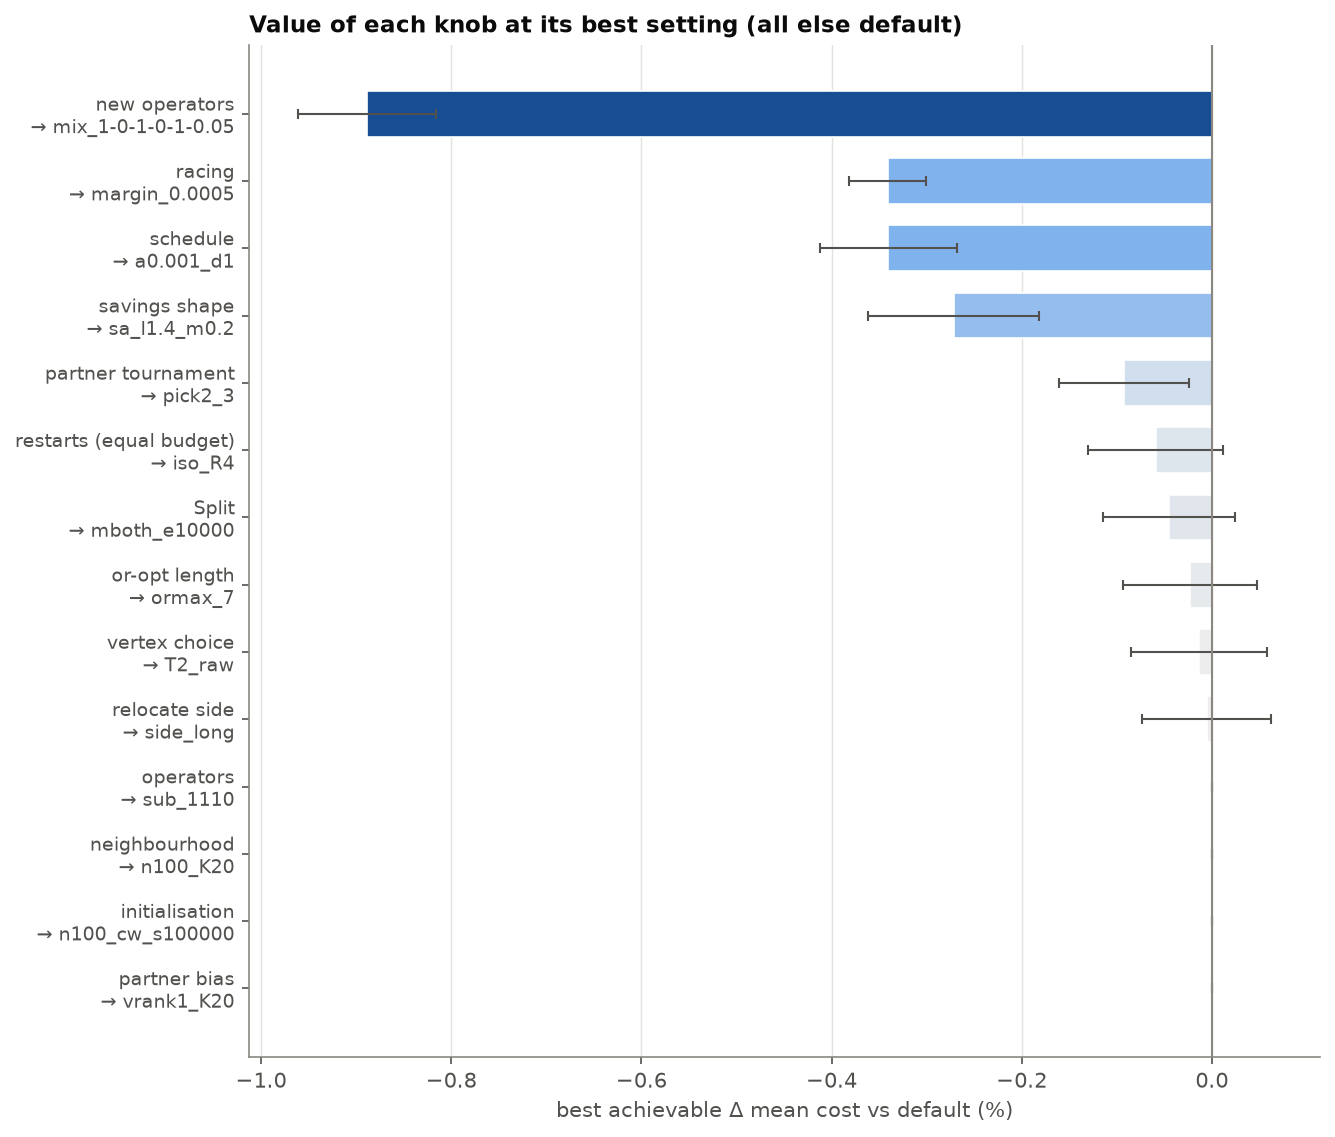
\includegraphics[width=\linewidth,height=0.74\textheight,keepaspectratio]{figures/overview.png}
  \caption{Best achievable improvement per knob, with 95\,\% CIs. Bars that cross zero are knobs with no measurable effect on this instance family at this budget.}
\end{figure}

\begin{table}[H]\centering\small
\begin{tabular}{llrrr}
\toprule
\textbf{knob} & \textbf{best setting found} & \textbf{$\Delta$ (\%)} & \textbf{95\,\% CI} & \textbf{win/loss} \\
\midrule
  new operators & \texttt{mix\_1-0-1-0-1-0.05} & \textbf{-0.889} & [-0.961,\;-0.817] & 780/219 \\
  racing & \texttt{margin\_0.0005} & \textbf{-0.341} & [-0.381,\;-0.300] & 658/261 \\
  schedule & \texttt{a0.001\_d1} & \textbf{-0.340} & [-0.413,\;-0.268] & 610/384 \\
  savings shape & \texttt{sa\_l1.4\_m0.2} & \textbf{-0.272} & [-0.362,\;-0.182] & 569/431 \\
  partner tournament & \texttt{pick2\_3} & \textbf{-0.092} & [-0.161,\;-0.024] & 538/457 \\
  restarts (equal budget) & \texttt{iso\_R4} & -0.059 & [-0.130,\;+0.012] & 504/495 \\
  Split & \texttt{mboth\_e10000} & -0.045 & [-0.115,\;+0.025] & 498/496 \\
  or-opt length & \texttt{ormax\_7} & -0.023 & [-0.094,\;+0.047] & 527/467 \\
  vertex choice & \texttt{T2\_raw} & -0.014 & [-0.085,\;+0.058] & 508/488 \\
  relocate side & \texttt{side\_long} & -0.006 & [-0.074,\;+0.063] & 496/496 \\
  operators & \texttt{sub\_1110} & +0.000 & [+0.000,\;+0.000] & 0/0 \\
  neighbourhood & \texttt{n100\_K20} & +0.000 & [+0.000,\;+0.000] & 0/0 \\
  initialisation & \texttt{n100\_cw\_s100000} & +0.000 & [+0.000,\;+0.000] & 0/0 \\
  partner bias & \texttt{vrank1\_K20} & +0.000 & [+0.000,\;+0.000] & 0/0 \\
\bottomrule
\end{tabular}
\caption{Each knob at its best setting, paired against its own default.}
\end{table}


\section{Initialisation: where the annealing starts from}\label{sec:init}

\textbf{What it controls.} \texttt{-{}-init} chooses the solution the simulated
annealing starts from. \texttt{cw} (the default) runs the Clarke \& Wright
savings construction: every pair of customers gets a score
$s(i,j) = d_{0i} + d_{0j} - \lambda\,d_{ij} + \mu\,|d_{0i}-d_{0j}|$, measuring how
much is saved by serving $i$ and $j$ on one route instead of two, and merges
route endpoints greedily in decreasing score while capacity allows.
\texttt{random} throws that away: it shuffles the customers and cuts the
permutation into routes at the capacity limit (first fit). Under
\texttt{-{}-restarts} each restart draws its own permutation.

\textbf{The question.} A random start is $100$--$380\,\%$ worse before annealing.
Does the annealing erase that, and how much budget does it cost to do so?

\begin{figure}[H]\centering
  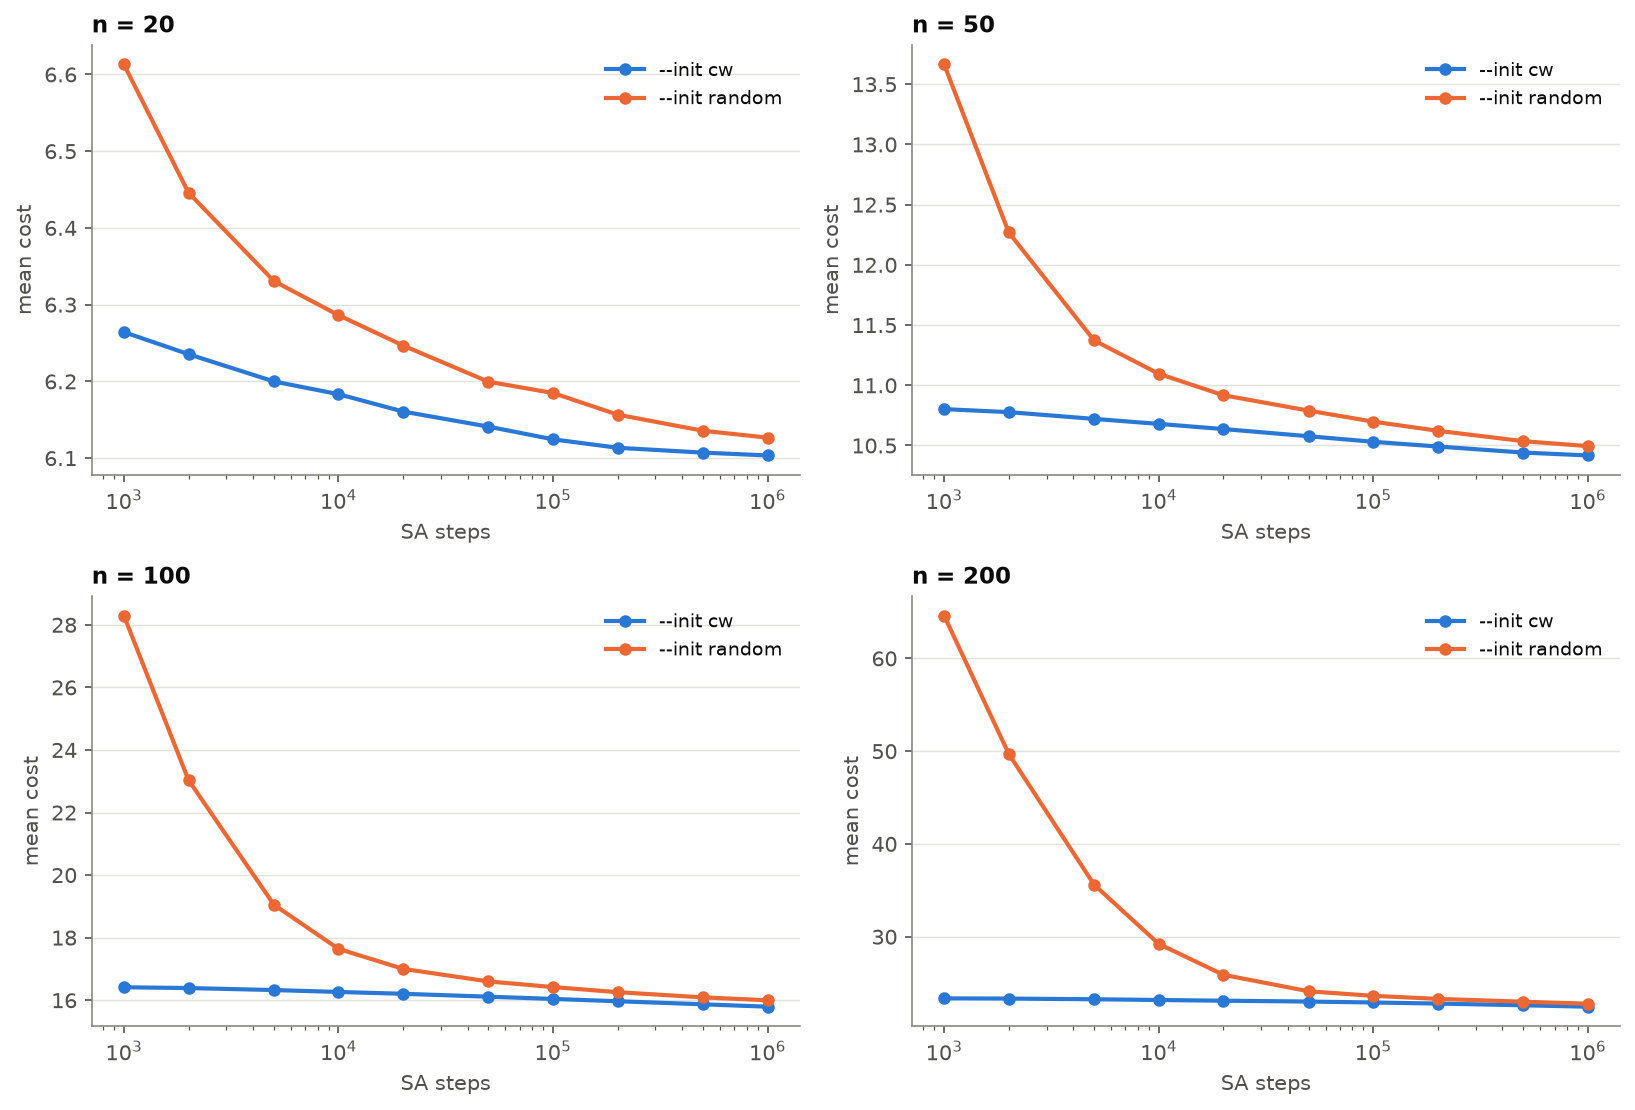
\includegraphics[width=\linewidth,height=0.74\textheight,keepaspectratio]{figures/init_curves.png}
  \caption{Mean cost against the annealing budget, for both initialisations, at four dimensions. Same budget on both sides of each panel.}
\end{figure}

\begin{figure}[H]\centering
  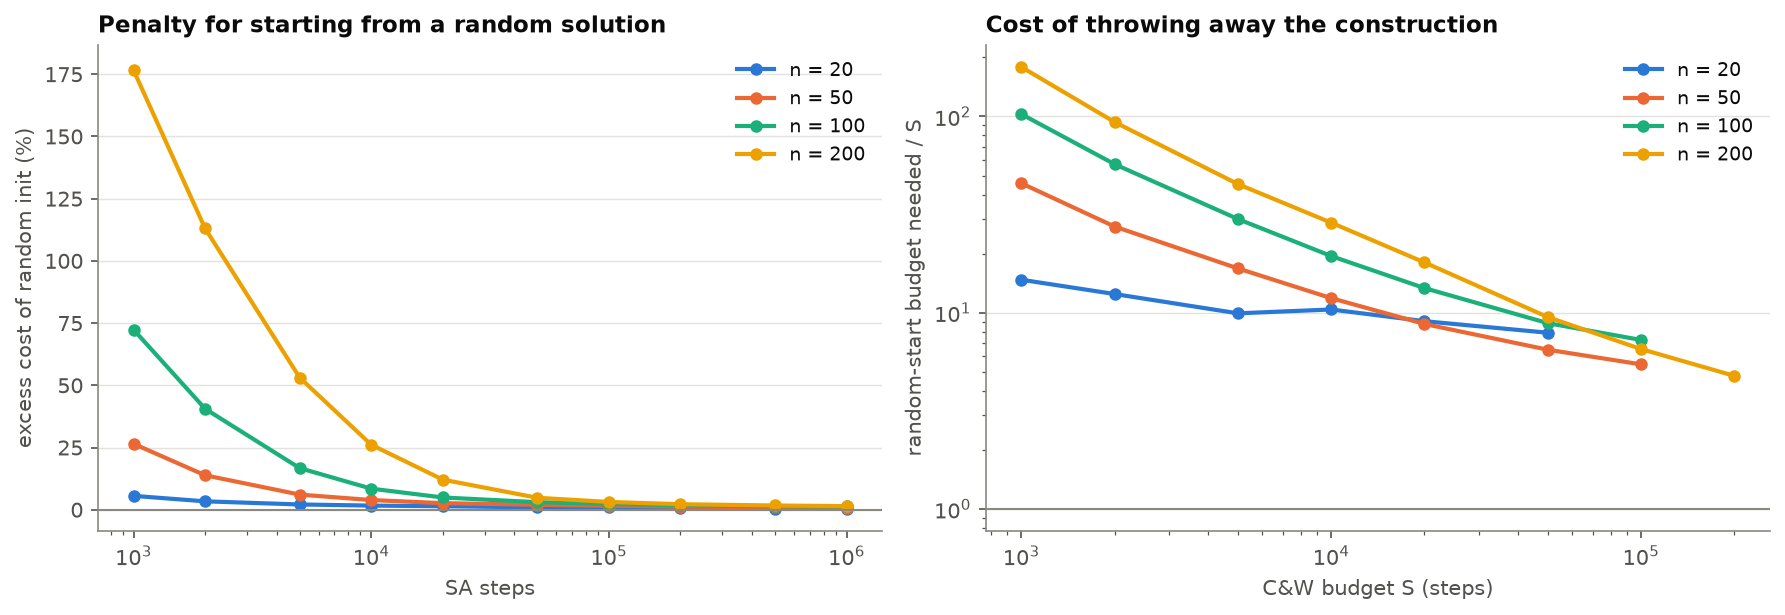
\includegraphics[width=\linewidth,height=0.74\textheight,keepaspectratio]{figures/init_gap.png}
  \caption{Left: paired excess of the random start over Clarke \& Wright at equal budget, with a 95\,\% band. Right: how many steps the random start needs to reach what Clarke \& Wright reaches at $S$ steps.}
\end{figure}

\begin{table}[H]\centering\small
\begin{tabular}{rrrr}
\toprule
\textbf{$n$} & \textbf{excess at $10^3$ (\%)} & \textbf{excess at $10^6$ (\%)} & \textbf{steps to catch up} \\
\midrule
  20 & +5.57 & +0.38 & not within $10^6$ \\
  50 & +26.49 & +0.74 & not within $10^6$ \\
  100 & +72.36 & +1.30 & not within $10^6$ \\
  200 & +176.60 & +1.44 & not within $10^6$ \\
\bottomrule
\end{tabular}
\caption{Penalty for a random start, paired against the C\&W start at the same budget. `Catch up' is the first budget at which the upper end of the 95\,\% CI reaches zero.}
\end{table}

\begin{table}[H]\centering\small
\begin{tabular}{rrrr}
\toprule
\textbf{$n$} & \textbf{at smallest $S$} & \textbf{mid-range $S$} & \textbf{at largest $S$} \\
\midrule
  20 & 15$\times$ & 10$\times$ & 8$\times$ \\
  50 & 46$\times$ & 12$\times$ & 5$\times$ \\
  100 & 103$\times$ & 19$\times$ & 7$\times$ \\
  200 & 179$\times$ & 18$\times$ & 5$\times$ \\
\bottomrule
\end{tabular}
\caption{Budget multiplier: steps the random start needs to match the C\&W start, relative to the C\&W budget. A ratio of 1 means the head start has been fully repaid.}
\end{table}

\textbf{Reading.} The random start converges to parity but never overtakes: it
buys no extra diversity that the annealing can exploit. The gap closes late and
costs dearly along the way --- at $n=200$ it still needs several times the budget
at $10^5$ steps. Keep the construction.


\section{Move operators}\label{sec:ops}

\textbf{What it controls.} \texttt{-{}-ops r,s,t,o} sets the relative
probabilities of the four neighbourhood moves the annealing draws from. Each
move first picks a vertex $u$ (Section~\ref{sec:pick}) and a partner $v$ near it
(Section~\ref{sec:knn}), then:
\begin{itemize}\itemsep2pt
  \item \textbf{relocate} (\texttt{mv\_relocate}, \texttt{cw.c:1040}) --- take $u$
        out of its route and re-insert it next to $v$, possibly in another route.
  \item \textbf{swap} (\texttt{mv\_swap}, \texttt{cw.c:1083}) --- exchange the
        positions of $u$ and $v$.
  \item \textbf{2-opt} (\texttt{mv\_2opt}, \texttt{cw.c:1362}) --- replace the two
        edges carried by $u$ and $v$ by the other pairing; inside one route this
        reverses a segment, across two routes it exchanges their tails.
  \item \textbf{or-opt} (\texttt{mv\_oropt}, \texttt{cw.c:1148}) --- move a whole
        run of 2 to \texttt{-{}-or-max} consecutive customers starting at $u$,
        optionally reversed, next to $v$.
\end{itemize}
Every move is accepted by the Metropolis rule on its exact cost delta. The
default is \texttt{1,1,1,0}: or-opt is present in the code but switched off.
\texttt{-{}-ops} takes two further weights, for swap* and route opening, which
are also zero by default and have a section of their own
(Section~\ref{sec:newops}); this section is about the original four, so every
run in it leaves the other two at zero.

\textbf{The question.} Is the default subset the right one, is the uniform
weighting right, and is or-opt off for a good reason?

\begin{figure}[H]\centering
  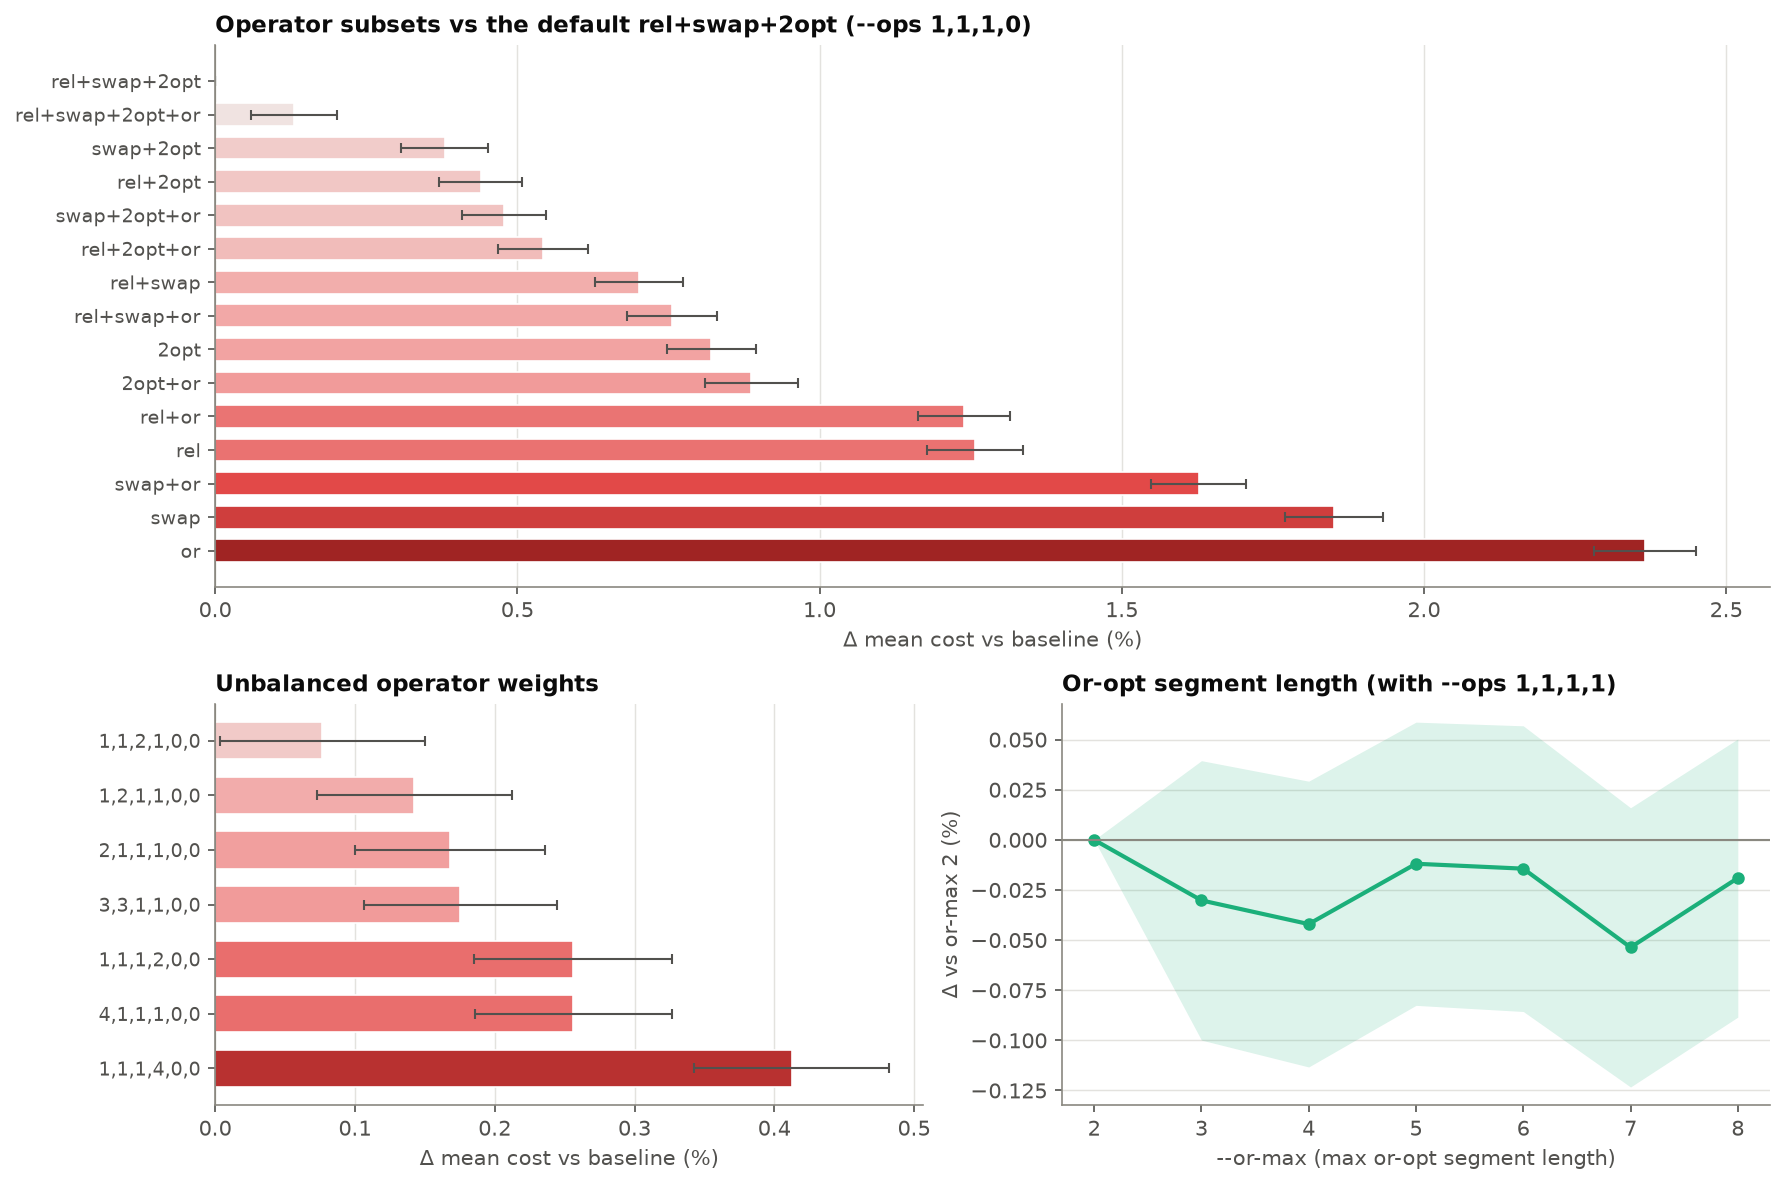
\includegraphics[width=\linewidth,height=0.74\textheight,keepaspectratio]{figures/ops.png}
  \caption{Top: all 15 non-empty operator subsets. Bottom left: unbalanced weightings. Bottom right: the or-opt segment length cap. Bars are paired deltas against the default with 95\,\% CIs.}
\end{figure}

\begin{table}[H]\centering\small
\begin{tabular}{lrrrr}
\toprule
\textbf{subset} & \textbf{mean cost} & \textbf{$\Delta$ (\%)} & \textbf{95\,\% CI} & \textbf{win/loss} \\
\midrule
  rel+swap+2opt & 16.04122 & +0.000 & [+0.000,\;+0.000] & 0/0 \\
  rel+swap+2opt+or & 16.06218 & +0.131 & [+0.060,\;+0.201] & 470/525 \\
  swap+2opt & 16.10209 & \textbf{+0.379} & [+0.307,\;+0.452] & 369/627 \\
  rel+2opt & 16.11166 & \textbf{+0.439} & [+0.370,\;+0.508] & 342/653 \\
  swap+2opt+or & 16.11796 & \textbf{+0.478} & [+0.409,\;+0.548] & 329/666 \\
  rel+2opt+or & 16.12824 & \textbf{+0.542} & [+0.469,\;+0.616] & 314/683 \\
  rel+swap & 16.15369 & \textbf{+0.701} & [+0.628,\;+0.774] & 270/725 \\
  rel+swap+or & 16.16246 & \textbf{+0.756} & [+0.681,\;+0.831] & 250/744 \\
  2opt & 16.17295 & \textbf{+0.821} & [+0.747,\;+0.895] & 248/750 \\
  2opt+or & 16.18348 & \textbf{+0.887} & [+0.810,\;+0.964] & 223/773 \\
  rel+or & 16.23998 & \textbf{+1.239} & [+1.163,\;+1.315] & 137/861 \\
  rel & 16.24291 & \textbf{+1.257} & [+1.178,\;+1.336] & 156/841 \\
  swap+or & 16.30221 & \textbf{+1.627} & [+1.548,\;+1.706] & 75/913 \\
  swap & 16.33812 & \textbf{+1.851} & [+1.769,\;+1.932] & 39/947 \\
  or & 16.42064 & \textbf{+2.365} & [+2.281,\;+2.450] & 9/977 \\
\bottomrule
\end{tabular}
\caption{All 15 non-empty operator subsets, paired against the default \texttt{-{}-ops 1,1,1,0}. Bold = significant at 95\,\% and by sign test.}
\end{table}

\begin{table}[H]\centering\small
\begin{tabular}{lrrrr}
\toprule
\textbf{weights} & \textbf{mean cost} & \textbf{$\Delta$ (\%)} & \textbf{95\,\% CI} & \textbf{win/loss} \\
\midrule
  \texttt{1,1,2,1,0,0} & 16.05353 & +0.077 & [+0.004,\;+0.150] & 470/528 \\
  \texttt{1,2,1,1,0,0} & 16.06408 & \textbf{+0.143} & [+0.073,\;+0.212] & 442/550 \\
  \texttt{2,1,1,1,0,0} & 16.06813 & \textbf{+0.168} & [+0.100,\;+0.236] & 433/563 \\
  \texttt{3,3,1,1,0,0} & 16.06933 & \textbf{+0.175} & [+0.106,\;+0.244] & 447/548 \\
  \texttt{1,1,1,2,0,0} & 16.08225 & \textbf{+0.256} & [+0.185,\;+0.327] & 410/585 \\
  \texttt{4,1,1,1,0,0} & 16.08233 & \textbf{+0.256} & [+0.186,\;+0.327] & 426/568 \\
  \texttt{1,1,1,4,0,0} & 16.10738 & \textbf{+0.412} & [+0.342,\;+0.482] & 349/646 \\
\bottomrule
\end{tabular}
\caption{Unbalanced weightings, against the same default.}
\end{table}

\begin{table}[H]\centering\small
\begin{tabular}{rrrrr}
\toprule
\textbf{\texttt{-{}-or-max}} & \textbf{mean cost} & \textbf{$\Delta$ (\%)} & \textbf{95\,\% CI} & \textbf{win/loss} \\
\midrule
  2 & 16.06703 & +0.000 & [+0.000,\;+0.000] & 0/0 \\
  3 & 16.06218 & -0.030 & [-0.100,\;+0.039] & 524/474 \\
  4 & 16.06028 & -0.042 & [-0.113,\;+0.029] & 512/486 \\
  5 & 16.06512 & -0.012 & [-0.083,\;+0.059] & 519/478 \\
  6 & 16.06472 & -0.014 & [-0.086,\;+0.057] & 486/510 \\
  7 & 16.05841 & -0.054 & [-0.123,\;+0.016] & 530/465 \\
  8 & 16.06397 & -0.019 & [-0.088,\;+0.050] & 508/488 \\
\bottomrule
\end{tabular}
\caption{Or-opt segment length, with or-opt enabled (\texttt{-{}-ops 1,1,1,1}). Valid range is 2--8 (\texttt{cw.c:2546}).}
\end{table}

\textbf{Reading.} The default subset wins: every other subset is worse, and
turning or-opt on costs a small but significant amount. Or-opt overlaps with
relocate (a length-1 relocate is the same move) while being more expensive per
draw, so at a fixed step count it buys less. \texttt{-{}-or-max} is then
irrelevant --- its whole range sits inside the noise. Leaving or-opt off is the
right default.


\section{swap* and route opening}\label{sec:newops}

\textbf{What it controls.} \texttt{-{}-ops} carries two further weights beyond
the four of Section~\ref{sec:ops}, both defaulting to zero:
\begin{itemize}\itemsep2pt
  \item \textbf{swap*} (\texttt{mv\_swapstar}, \texttt{cw.c:1216}) --- Vidal's
        \emph{Hybrid genetic search for the CVRP}, C\&OR 2022. Ordinary swap
        forces $u$ into $v$'s slot; swap* drops that and re-inserts each of the
        two customers at its \emph{best} position in the other's route. The two
        routes are disjoint, so the two re-insertions are independent and the
        delta is still exact --- but the scan costs $O(L_1+L_2)$ instead of
        $O(1)$. The kNN neighbour selects the target \emph{route}, not the
        partner: $v$ is then the worse by regret of two uniform customers of
        that route.
  \item \textbf{opening} (\texttt{mv\_open}, \texttt{cw.c:1325}) --- isolate one
        customer in an empty route. Almost always worsening, and that is the
        point: the annealing can empty a route but has no move that repopulates
        one, so the number of active routes is a one-way door between two
        Splits. This is the only move that opens it again.
\end{itemize}

\textbf{The question.} swap* is the one non-elementary operator in the solver,
so it has to earn its cost: at a fixed step count it is not competing on equal
terms. Everything below is therefore also measured against wall time.

\begin{figure}[H]\centering
  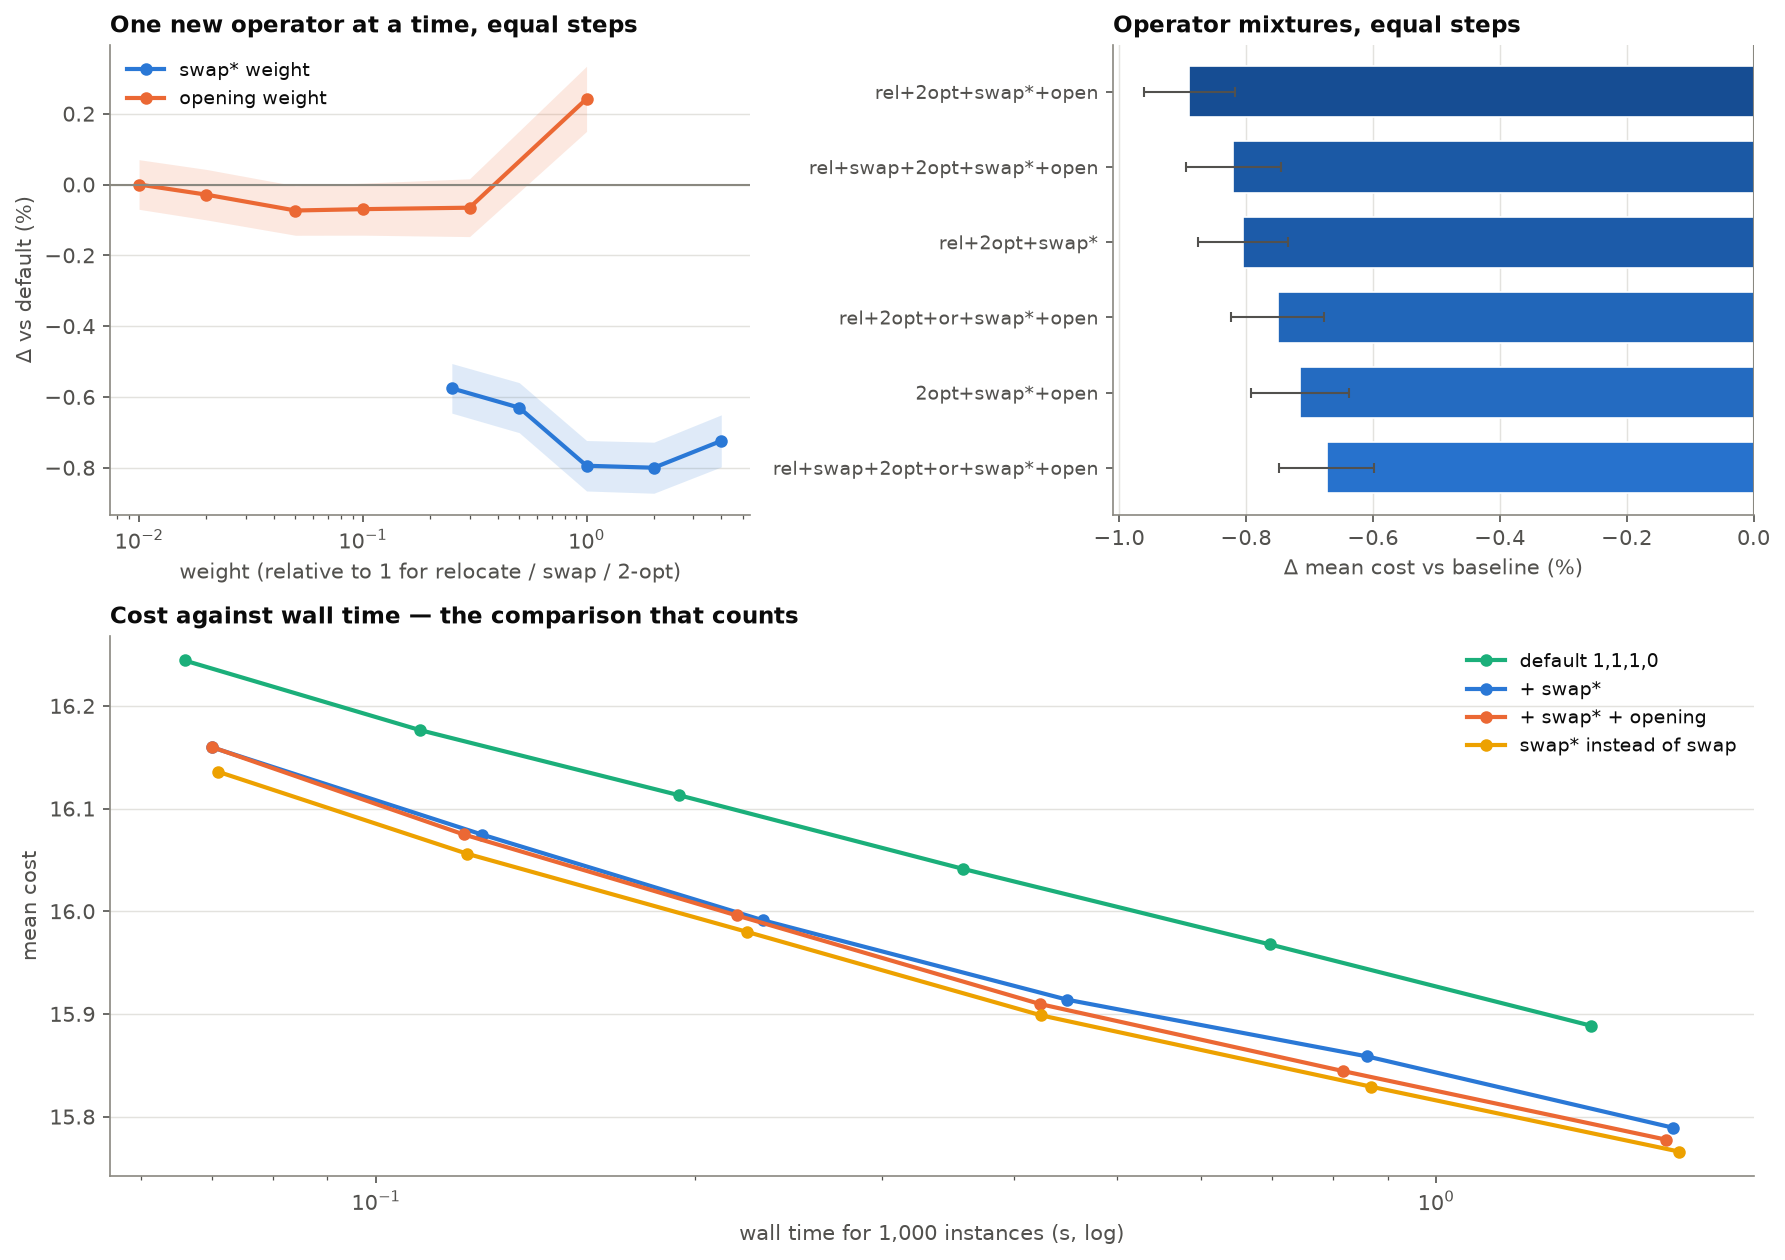
\includegraphics[width=\linewidth,height=0.74\textheight,keepaspectratio]{figures/newops.png}
  \caption{Top left: each new operator's weight swept alone. Top right: mixtures. Bottom: cost against measured wall time for four configurations swept over a 32x budget range --- a curve that sits lower-left dominates.}
\end{figure}

\begin{table}[H]\centering\small
\begin{tabular}{lrrrr}
\toprule
\textbf{mixture} & \textbf{mean cost} & \textbf{$\Delta$ (\%)} & \textbf{95\,\% CI} & \textbf{win/loss} \\
\midrule
  rel+2opt+swap*+open & 15.89863 & \textbf{-0.889} & [-0.961,\;-0.817] & 780/219 \\
  rel+swap+2opt+swap*+open & 15.90965 & \textbf{-0.820} & [-0.895,\;-0.745] & 762/236 \\
  rel+2opt+swap* & 15.91220 & \textbf{-0.804} & [-0.875,\;-0.734] & 790/210 \\
  rel+2opt+or+swap*+open & 15.92089 & \textbf{-0.750} & [-0.823,\;-0.677] & 725/270 \\
  2opt+swap*+open & 15.92661 & \textbf{-0.714} & [-0.792,\;-0.637] & 717/282 \\
  rel+swap+2opt+or+swap*+open & 15.93332 & \textbf{-0.673} & [-0.747,\;-0.598] & 719/280 \\
\bottomrule
\end{tabular}
\caption{Operator mixtures at equal step count, paired against the stock \texttt{-{}-ops 1,1,1,0,0,0}. Equal steps flatters swap*, which is why the wall-time reading below is the one to trust.}
\end{table}

\begin{table}[H]\centering\small
\begin{tabular}{lrrrrrrrr}
\toprule
\textbf{configuration} & \textbf{time} & \textbf{default} & \textbf{this} & \textbf{$\Delta$} & \textbf{time} & \textbf{default} & \textbf{this} & \textbf{$\Delta$} \\
\midrule
  + swap* & 0.36s & 16.04122 & 15.94030 & -0.629\,\% & 1.40s & 15.88861 & 15.80788 & -0.508\,\% \\
  + swap* + opening & 0.36s & 16.04122 & 15.93151 & -0.684\,\% & 1.40s & 15.88861 & 15.79315 & -0.601\,\% \\
  swap* instead of swap & 0.36s & 16.04122 & 15.92016 & -0.755\,\% & 1.40s & 15.88861 & 15.78408 & -0.658\,\% \\
\bottomrule
\end{tabular}
\caption{Iso-time reading of the bottom panel: both curves interpolated in $\log$(wall time) at two points of the default's own ladder. Negative $\Delta$ = better at the same wall time.}
\end{table}

\begin{table}[H]\centering\small
\begin{tabular}{rrrrrrr}
\toprule
\textbf{$n$} & \textbf{default} & \textbf{+swap*+open} & \textbf{$\Delta$ (\%)} & \textbf{95\,\% CI} & \textbf{win/loss} & \textbf{time x} \\
\midrule
  20 & 6.12446 & 6.11696 & \textbf{-0.122} & [-0.182,\;-0.062] & 237/144 & 1.23 \\
  50 & 10.53078 & 10.47592 & \textbf{-0.521} & [-0.614,\;-0.428] & 609/327 & 1.19 \\
  100 & 16.04122 & 15.90965 & \textbf{-0.820} & [-0.895,\;-0.745] & 762/236 & 1.18 \\
  200 & 22.91368 & 22.66046 & \textbf{-1.105} & [-1.167,\;-1.043] & 880/120 & 1.20 \\
  500 & 39.05297 & 38.78281 & \textbf{-0.692} & [-0.724,\;-0.660] & 923/77 & 1.14 \\
\bottomrule
\end{tabular}
\caption{\texttt{-{}-ops 1,1,1,0,1,0.05} against the default across dimension, at equal step count. The last column is the wall time ratio --- the price of the equal-step gain.}
\end{table}

\textbf{Reading.} swap* is the largest single improvement in this whole
document, and --- unlike most of the others --- it survives the change of
yardstick. It costs about 20\,\% more wall time per step, but the iso-time table
shows it still ahead by roughly half a percent at both ends of the ladder, so
the extra work per draw is bought back several times over. Its weight is
insensitive over the whole range tried: anything from a quarter to four times
the weight of relocate lands within noise of the same place, which is what one
wants from a knob.

Route opening is a different kind of thing. On its own it is worth almost
nothing, and at large weight it is actively harmful --- unsurprising, since it
never improves a solution by itself. It is a pure enabler: the annealing can
empty a route but has no other move that repopulates one, so without it the
route count is monotone between two Splits. Kept at a small weight it is close
to free and slightly positive.

The one result here that contradicts the intuition behind the code is that
\emph{dropping} swap in favour of swap* is not a trade-off at all: it is the
best configuration on the ladder at both time points. For any given pair, the
in-place exchange is one of the positions swap* already sweeps, so
$\Delta_{\text{swap*}} \le \Delta_{\text{swap}}$ always; the measurement says
that the ten-fold cheaper draw of ordinary swap does not buy back that
domination. swap is nevertheless kept in the code as a separate operator --- it
is a weighting decision, and \texttt{-{}-ops 1,1,1,0,1,0.05} remains the safer
recommendation at small $n$, where the two are within noise of each other.


\section{Candidate neighbourhood}\label{sec:knn}

\textbf{What it controls.} Once a move has picked the vertex $u$, it needs a
partner $v$. \texttt{sa\_cand} (\texttt{cw.c:1010}) draws $v$ uniformly from the
$K$ nearest neighbours of $u$, with $K=$ \texttt{-{}-sa-knn}; at $K=0$ it draws
uniformly from all customers. This is what keeps a move geometrically local, so
that the cost delta has a chance of being negative. $K$ is clamped to $n-1$
(\texttt{cw.c:1675}).

\begin{quote}\small $K$ does double duty: at $K=0$ the kNN lists are not built, and
\texttt{cw.c:1676} then \emph{silently} forces uniform vertex selection as well,
whatever \texttt{-{}-pick} says. So $K=0$ disables two mechanisms, not one ---
see Section~\ref{sec:pick}.\end{quote}

\begin{figure}[H]\centering
  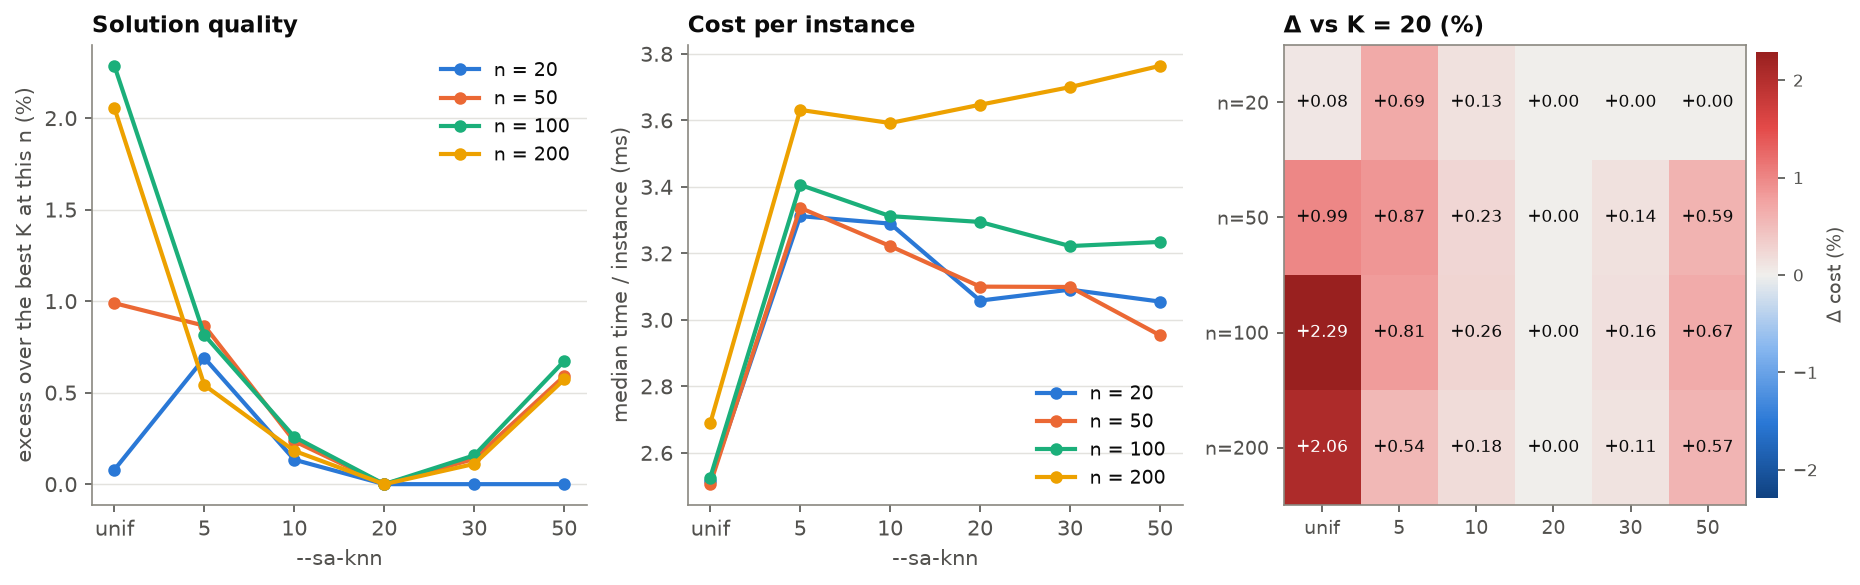
\includegraphics[width=\linewidth,height=0.74\textheight,keepaspectratio]{figures/knn.png}
  \caption{Quality (left, as excess over the best $K$ at that $n$), cost per instance (middle) and the paired delta against $K=20$ (right).}
\end{figure}

{\small\begin{longtable}{rrrrrrrrl}
\caption{\texttt{-{}-sa-knn} across dimension, paired against $K=20$. The effective $K$ is $\min(K, n-1)$, which is why the rows for $n=20$ at $K \ge 20$ are exactly identical runs.}\\
\toprule
\textbf{$n$} & \textbf{$K$} & \textbf{effective $K$} & \textbf{mean cost} & \textbf{$\Delta$ (\%)} & \textbf{95\,\% CI} & \textbf{win/loss} & \textbf{ms/inst} & \textbf{} \\
\midrule
\endfirsthead
\toprule
\textbf{$n$} & \textbf{$K$} & \textbf{effective $K$} & \textbf{mean cost} & \textbf{$\Delta$ (\%)} & \textbf{95\,\% CI} & \textbf{win/loss} & \textbf{ms/inst} & \textbf{} \\
\midrule
\endhead
  20 & 0 & uniform & 6.12929 & \textbf{+0.079} & [+0.014,\;+0.144] & 182/238 & 2.516 &  \\
  20 & 5 & 5 & 6.16670 & \textbf{+0.690} & [+0.582,\;+0.797] & 136/370 & 3.312 &  \\
  20 & 10 & 10 & 6.13264 & +0.134 & [+0.063,\;+0.205] & 192/202 & 3.290 &  \\
  20 & 20 & 19 & 6.12446 & +0.000 & [+0.000,\;+0.000] & 0/0 & 3.058 & $\star$ \\
  20 & 30 & 19 & 6.12446 & +0.000 & [+0.000,\;+0.000] & 0/0 & 3.091 &  \\
  20 & 50 & 19 & 6.12446 & +0.000 & [+0.000,\;+0.000] & 0/0 & 3.055 &  \\
  50 & 0 & uniform & 10.63491 & \textbf{+0.989} & [+0.880,\;+1.097] & 241/714 & 2.506 &  \\
  50 & 5 & 5 & 10.62195 & \textbf{+0.866} & [+0.767,\;+0.965] & 257/699 & 3.337 &  \\
  50 & 10 & 10 & 10.55551 & \textbf{+0.235} & [+0.146,\;+0.324] & 419/514 & 3.222 &  \\
  50 & 20 & 20 & 10.53078 & +0.000 & [+0.000,\;+0.000] & 0/0 & 3.100 & $\star$ \\
  50 & 30 & 30 & 10.54532 & \textbf{+0.138} & [+0.040,\;+0.236] & 407/548 & 3.099 &  \\
  50 & 50 & 49 & 10.59292 & \textbf{+0.590} & [+0.484,\;+0.696] & 331/623 & 2.954 &  \\
  100 & 0 & uniform & 16.40787 & \textbf{+2.286} & [+2.202,\;+2.370] & 12/968 & 2.526 &  \\
  100 & 5 & 5 & 16.17189 & \textbf{+0.815} & [+0.742,\;+0.887] & 239/758 & 3.406 &  \\
  100 & 10 & 10 & 16.08260 & \textbf{+0.258} & [+0.190,\;+0.326] & 406/590 & 3.312 &  \\
  100 & 20 & 20 & 16.04122 & +0.000 & [+0.000,\;+0.000] & 0/0 & 3.295 & $\star$ \\
  100 & 30 & 30 & 16.06646 & \textbf{+0.157} & [+0.079,\;+0.236] & 434/558 & 3.222 &  \\
  100 & 50 & 50 & 16.14911 & \textbf{+0.673} & [+0.588,\;+0.757] & 292/696 & 3.234 &  \\
  200 & 0 & uniform & 23.38459 & \textbf{+2.055} & [+1.997,\;+2.113] & 0/995 & 2.689 &  \\
  200 & 5 & 5 & 23.03763 & \textbf{+0.541} & [+0.493,\;+0.589] & 232/768 & 3.631 &  \\
  200 & 10 & 10 & 22.95534 & \textbf{+0.182} & [+0.131,\;+0.233] & 420/580 & 3.592 &  \\
  200 & 20 & 20 & 22.91368 & +0.000 & [+0.000,\;+0.000] & 0/0 & 3.647 & $\star$ \\
  200 & 30 & 30 & 22.93903 & \textbf{+0.111} & [+0.057,\;+0.164] & 415/584 & 3.700 &  \\
  200 & 50 & 50 & 23.04476 & \textbf{+0.572} & [+0.513,\;+0.631] & 274/724 & 3.764 &  \\
\bottomrule
\end{longtable}}

\textbf{Reading.} $K=20$ is the optimum at every dimension tested, and the curve
is a clean U: too small a list starves the move of good partners, too large a
one dilutes it with distant ones that will be rejected. The default needs no
change --- and notably it does not need to grow with $n$.


\section{Compute cost}\label{sec:timing}

\textbf{What is measured.} Two phases: the Clarke \& Wright construction, which
builds a savings list ($O(n^2)$ exactly, for $n \le 1500$) and sorts it, and the
annealing, which does a fixed number of $O(1)$ steps regardless of $n$. Instances
are solved in parallel by OpenMP, one instance per thread, with no interaction
between them.

\begin{quote}\small \textbf{Metric: cumulative CPU time per instance, from the run log --- not the
\texttt{time\_ms} column of the CSV.} That column is wall time measured
\emph{inside} the 24-thread parallel region, so it absorbs memory contention: at
$n=1000$ it overstates the cost by about $2.5\times$ and is not additive, which
makes the annealing look roughly $10\times$ cheaper than it is. Use it for
latency distributions (third panel), never for cost accounting.\end{quote}

The annealing cost is isolated as $(t(10S) - t(S))/9$ at equal $n$: both runs pay
the same construction, so it cancels exactly. Construction is then $t(S)$ minus
that, cross-checked against an independent \texttt{-{}-no-sa} run. A $2\times$
budget delta was tried first and is not enough at $n=1000$, where the run-to-run
spread on the construction alone ($\pm 3\,\%$, measured over three repetitions)
exceeds the entire annealing cost.

\begin{table}[H]\centering\small
\begin{tabular}{rrrrrr}
\toprule
\textbf{$n$} & \textbf{construction} & \textbf{annealing} & \textbf{total} & \textbf{annealing share} & \textbf{\texttt{-{}-no-sa}} \\
\midrule
  20 & 0.0000 & 3.7639 & 3.6380 & 103.5\,\% & 0.0040 \\
  50 & 0.0119 & 3.7531 & 3.7650 & 99.7\,\% & 0.0180 \\
  100 & 0.8441 & 3.9319 & 4.7760 & 82.3\,\% & 0.0640 \\
  200 & 0.4082 & 4.0588 & 4.4670 & 90.9\,\% & 0.2250 \\
  500 & 2.7269 & 4.0681 & 6.7950 & 59.9\,\% & 1.2770 \\
  1000 & 5.4034 & 4.2526 & 9.6560 & 44.0\,\% & 4.5510 \\
\bottomrule
\end{tabular}
\caption{CPU time per instance (ms). Empirical scaling on this grid: construction $\sim n^{4.77}$, annealing $\sim n^{0.03}$ at a fixed step count --- the step count does not depend on $n$, so that exponent is pure cache behaviour.}
\end{table}

\begin{table}[H]\centering\small
\begin{tabular}{rrrr}
\toprule
\textbf{threads} & \textbf{wall (s)} & \textbf{speed-up} & \textbf{efficiency} \\
\midrule
  1 & 2.928 & 1.00$\times$ & 100\,\% \\
  2 & 1.482 & 1.98$\times$ & 99\,\% \\
  4 & 0.775 & 3.78$\times$ & 94\,\% \\
  8 & 0.385 & 7.61$\times$ & 95\,\% \\
  12 & 0.332 & 8.82$\times$ & 73\,\% \\
  16 & 0.328 & 8.93$\times$ & 56\,\% \\
  24 & 0.336 & 8.71$\times$ & 36\,\% \\
\bottomrule
\end{tabular}
\caption{Thread scaling at $n=100$. Instances are independent, so the loss at high thread counts is memory bandwidth and clock throttling, not synchronisation.}
\end{table}

\begin{figure}[H]\centering
  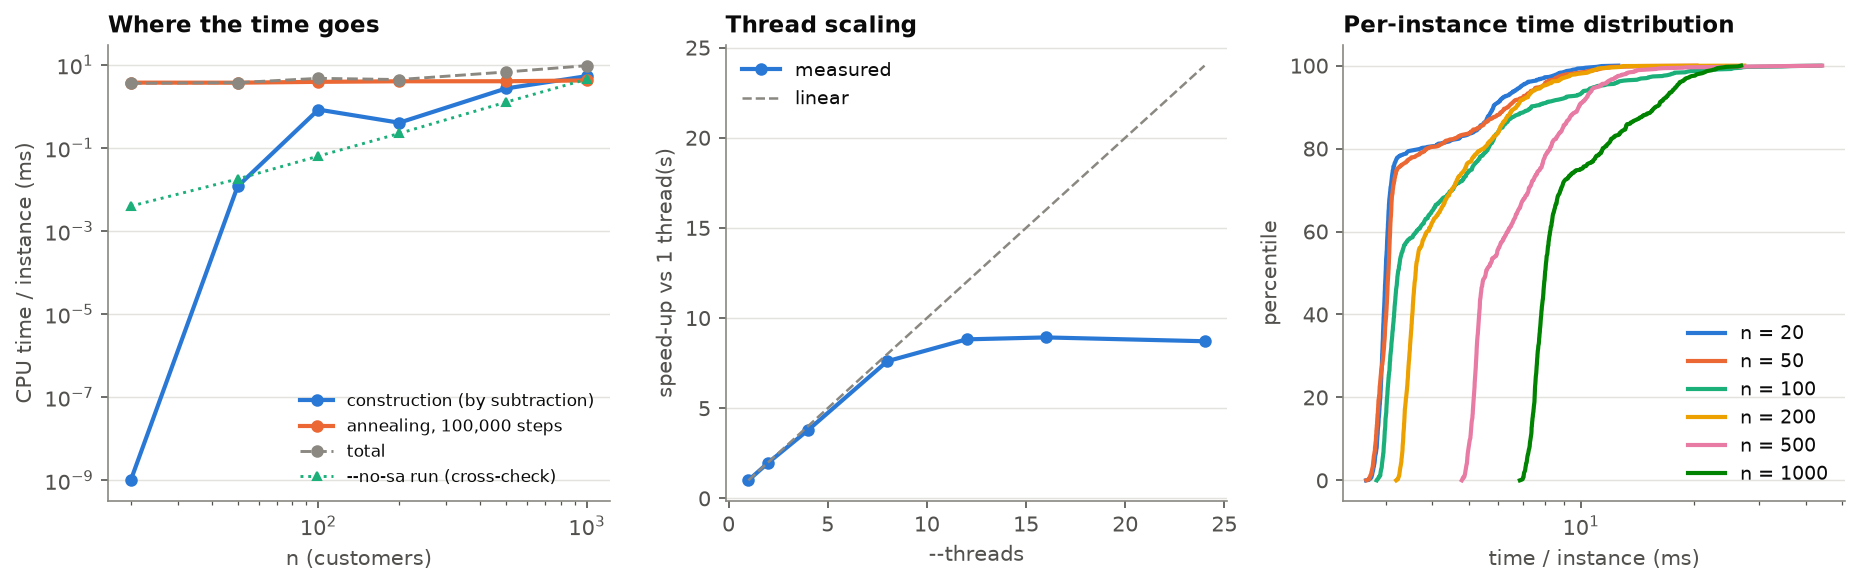
\includegraphics[width=\linewidth,height=0.74\textheight,keepaspectratio]{figures/timing.png}
  \caption{Left: construction and annealing cost against $n$ (log-log). Middle: thread scaling. Right: distribution of per-instance wall time inside the parallel region.}
\end{figure}

\textbf{Reading.} Up to $n \approx 200$ the annealing is essentially the whole
cost and the construction is free; past $n \approx 500$ the $O(n^2)$ savings list
takes over and dominates. If large instances ever become the target, the
construction is where to look --- \texttt{-{}-knn} truncates that list, and
Section~\ref{sec:construct} shows the annealing absorbs the loss of quality.


\section{Restarts}\label{sec:restarts}

\textbf{What it controls.} \texttt{-{}-restarts R} builds $R$ initial solutions
per instance, anneals each one, and keeps the best. Restart 0 is always the
deterministic Clarke \& Wright; the others are diversified by
\texttt{-{}-cw-rand}: \texttt{perturb} multiplies every saving by
$1 + \alpha\,U(-1,1)$ with $\alpha =$ \texttt{-{}-cw-alpha}, which reshuffles the
order in which pairs are merged; \texttt{param} redraws $\lambda$ and $\mu$;
\texttt{both} does both; \texttt{off} makes all restarts identical apart from
the annealing seed.

\begin{quote}\small \textbf{$R$ multiplies the work by $R$.} Comparing $R$ restarts against one at
the same \texttt{-{}-sa-steps} answers nothing useful --- of course more compute
helps. The study therefore also holds $R \times \texttt{sa-steps}$ constant, which
asks the question that matters: given a fixed number of annealing steps, is it
better to spend them on one long run or several short ones?\end{quote}

\begin{figure}[H]\centering
  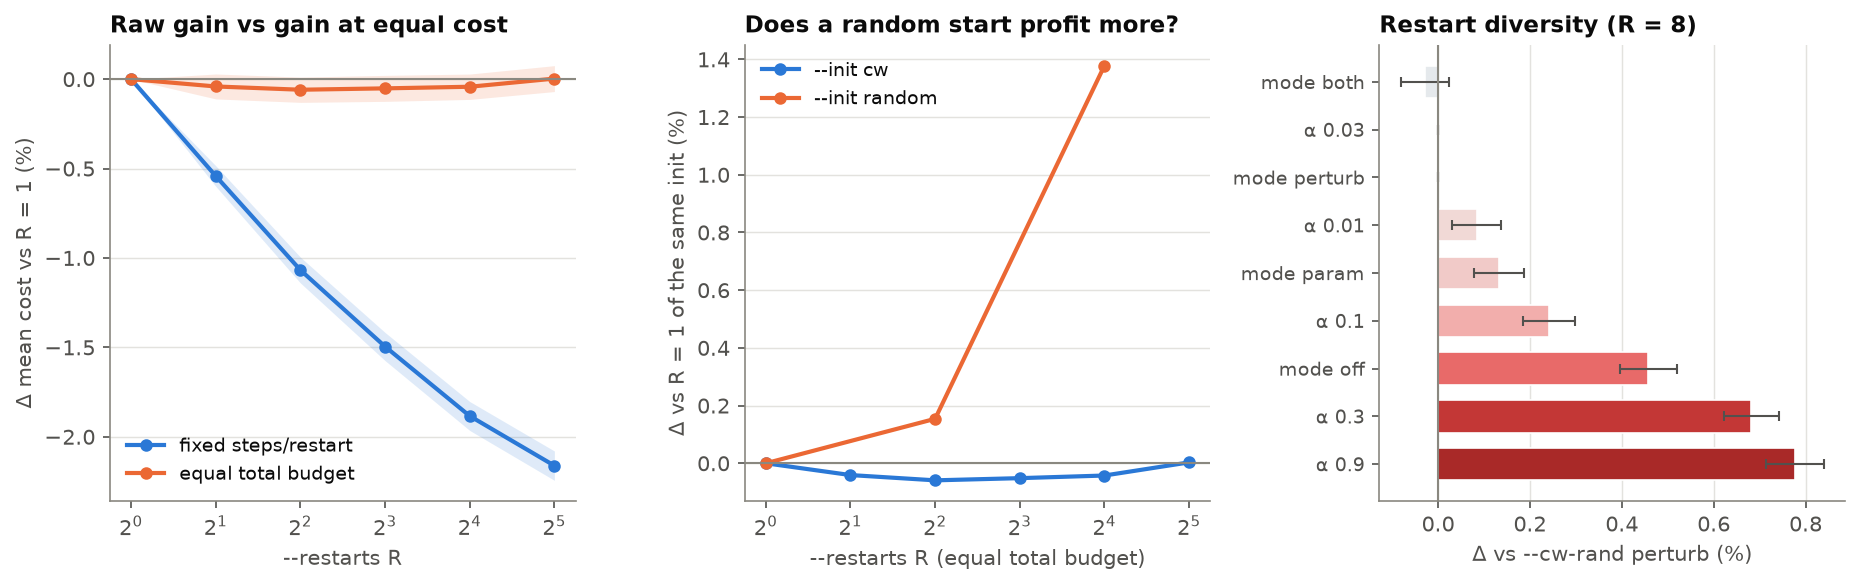
\includegraphics[width=\linewidth,height=0.74\textheight,keepaspectratio]{figures/restarts.png}
  \caption{Left: the same restart count judged two ways. Middle: restarts crossed with the initialisation. Right: how the diversity between restarts is generated.}
\end{figure}

\begin{table}[H]\centering\small
\begin{tabular}{rrrrrrr}
\toprule
\textbf{$R$} & \textbf{steps/restart} & \textbf{mean cost} & \textbf{$\Delta$ (\%)} & \textbf{95\,\% CI} & \textbf{win/loss} & \textbf{wall (s)} \\
\midrule
  1 & 320,000 & 15.91242 & +0.000 & [+0.000,\;+0.000] & 0/0 & 1.06 \\
  2 & 160,000 & 15.90591 & -0.041 & [-0.111,\;+0.029] & 497/501 & 1.06 \\
  4 & 80,000 & 15.90300 & -0.059 & [-0.130,\;+0.012] & 504/495 & 1.10 \\
  8 & 40,000 & 15.90421 & -0.052 & [-0.124,\;+0.021] & 489/510 & 1.13 \\
  16 & 20,000 & 15.90566 & -0.042 & [-0.113,\;+0.028] & 493/507 & 1.22 \\
  32 & 10,000 & 15.91291 & +0.003 & [-0.069,\;+0.076] & 482/518 & 1.38 \\
\bottomrule
\end{tabular}
\caption{Restarts at \emph{equal total budget} ($R \times \texttt{sa-steps} = 320\,000$), paired against $R=1$.}
\end{table}

\begin{table}[H]\centering\small
\begin{tabular}{rrrrrr}
\toprule
\textbf{$R$} & \textbf{mean cost} & \textbf{$\Delta$ (\%)} & \textbf{95\,\% CI} & \textbf{win/loss} & \textbf{wall (s)} \\
\midrule
  1 & 16.26449 & +0.000 & [+0.000,\;+0.000] & 0/0 & 0.06 \\
  2 & 16.17639 & \textbf{-0.542} & [-0.599,\;-0.484] & 435/0 & 0.10 \\
  4 & 16.09083 & \textbf{-1.068} & [-1.140,\;-0.996] & 715/0 & 0.18 \\
  8 & 16.02126 & \textbf{-1.495} & [-1.574,\;-1.417] & 853/0 & 0.35 \\
  16 & 15.95809 & \textbf{-1.884} & [-1.965,\;-1.803] & 937/0 & 0.68 \\
  32 & 15.91291 & \textbf{-2.162} & [-2.244,\;-2.080] & 974/0 & 1.37 \\
\bottomrule
\end{tabular}
\caption{Restarts at fixed steps per restart --- i.e.\ at $R$ times the compute. Shown for completeness; the table above is the meaningful one.}
\end{table}

\begin{table}[H]\centering\small
\begin{tabular}{lrrrr}
\toprule
\textbf{variant} & \textbf{mean cost} & \textbf{$\Delta$ (\%)} & \textbf{95\,\% CI} & \textbf{win/loss} \\
\midrule
  \texttt{mode both} & 15.89953 & -0.029 & [-0.082,\;+0.023] & 484/456 \\
  \texttt{alpha 0.03} & 15.90421 & +0.000 & [+0.000,\;+0.000] & 0/0 \\
  \texttt{mode perturb} & 15.90421 & +0.000 & [+0.000,\;+0.000] & 0/0 \\
  \texttt{alpha 0.01} & 15.91751 & \textbf{+0.084} & [+0.031,\;+0.137] & 439/502 \\
  \texttt{mode param} & 15.92521 & \textbf{+0.132} & [+0.077,\;+0.187] & 405/536 \\
  \texttt{alpha 0.1} & 15.94265 & \textbf{+0.242} & [+0.186,\;+0.298] & 360/559 \\
  \texttt{mode off} & 15.97703 & \textbf{+0.458} & [+0.396,\;+0.520] & 324/623 \\
  \texttt{alpha 0.3} & 16.01266 & \textbf{+0.682} & [+0.622,\;+0.742] & 160/728 \\
  \texttt{alpha 0.9} & 16.02768 & \textbf{+0.776} & [+0.713,\;+0.840] & 129/751 \\
\bottomrule
\end{tabular}
\caption{How restart diversity is produced, at $R=8$, against the default \texttt{perturb} with $\alpha=0.03$.}
\end{table}

\textbf{Reading.} At equal budget, restarts are flat: splitting $320\,000$ steps
into 2, 4, \dots, 32 independent anneals changes nothing significant. The
annealing is not getting trapped in a way that a fresh start would fix, so the
whole budget may as well go into one run. The random start is the exception ---
it degrades sharply as its share of the budget shrinks, which is the same result
as Section~\ref{sec:init} seen from another angle. On diversity, the default \texttt{perturb}
at $\alpha=0.03$ is the best of the options: too much perturbation
($\alpha \ge 0.3$) damages every restart, and \texttt{off} is worse still.


\section{Optimal Split}\label{sec:split}

\textbf{What it controls.} Split (Vidal, 2016) takes the current solution,
concatenates its routes into one giant tour ignoring capacity, then re-cuts that
tour into routes optimally by dynamic programming in $O(n)$. Because the current
partition is one of the candidates, the result can never be worse.
\texttt{-{}-split} says where to apply it: \texttt{cw} right after the
construction, \texttt{end} after the annealing, \texttt{both}, or \texttt{off}.
\texttt{-{}-split-every N} additionally applies it every $N$ annealing steps ---
an independent code path (\texttt{cw.c:1744} versus \texttt{cw.c:1968/2075}), so
\texttt{off} combined with a period is a meaningful cell. \texttt{-{}-split-tour}
chooses how the giant tour is built: routes in their current order,
\texttt{sweep} by polar angle, or \texttt{both} keeping the better.

\begin{figure}[H]\centering
  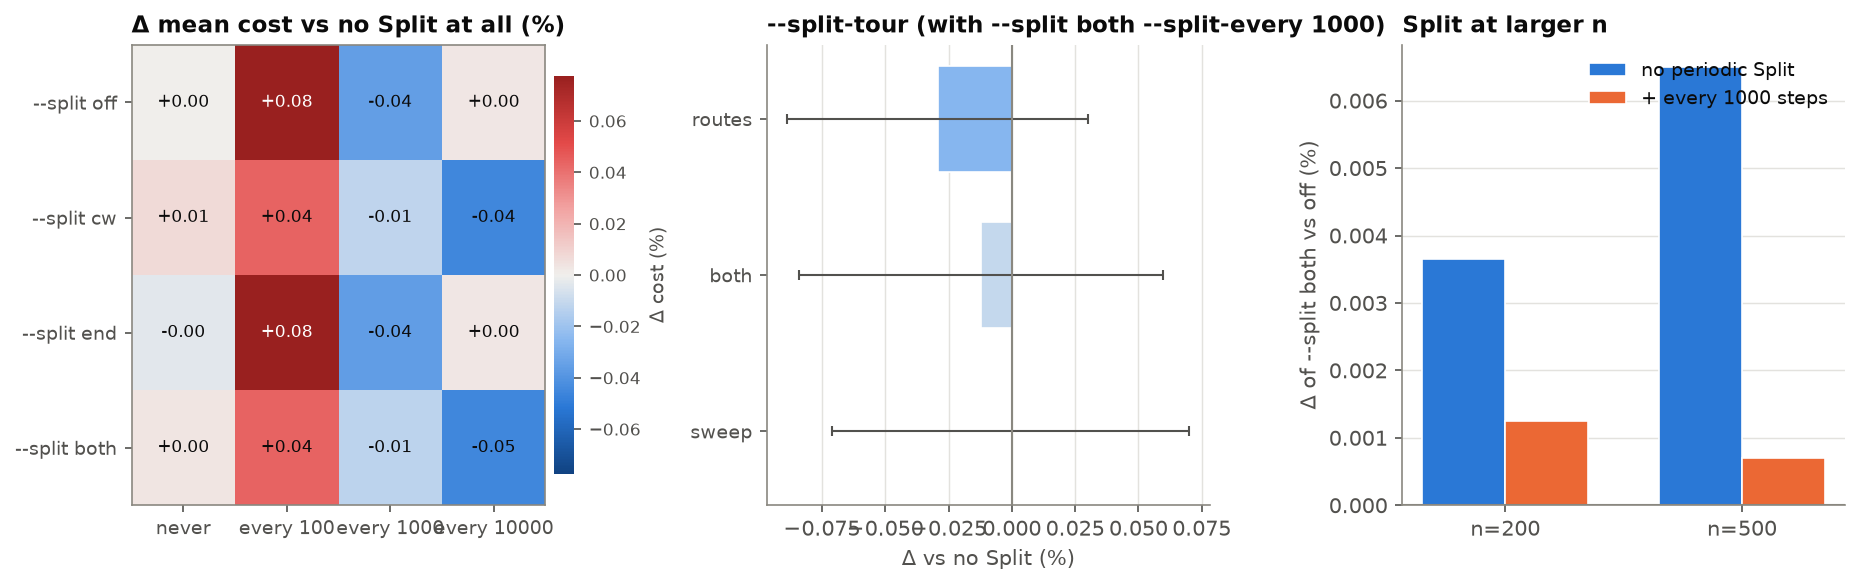
\includegraphics[width=\linewidth,height=0.74\textheight,keepaspectratio]{figures/split.png}
  \caption{Left: the full mode $\times$ period grid. Middle: giant-tour construction. Right: the same comparison at larger $n$, where there are more routes to repartition.}
\end{figure}

{\small\begin{longtable}{llrrrrrr}
\caption{Split mode against periodic Split, paired against no Split at all. `Split gain' is the total improvement cw attributes to Split internally --- note it is large where the paired delta is not, i.e.\ Split keeps recovering cost the annealing had just spent.}\\
\toprule
\textbf{\texttt{-{}-split}} & \textbf{\texttt{-{}-split-every}} & \textbf{mean cost} & \textbf{$\Delta$ (\%)} & \textbf{95\,\% CI} & \textbf{win/loss} & \textbf{Split gain} & \textbf{wall (s)} \\
\midrule
\endfirsthead
\toprule
\textbf{\texttt{-{}-split}} & \textbf{\texttt{-{}-split-every}} & \textbf{mean cost} & \textbf{$\Delta$ (\%)} & \textbf{95\,\% CI} & \textbf{win/loss} & \textbf{Split gain} & \textbf{wall (s)} \\
\midrule
\endhead
  \texttt{off} & never & 16.04122 & +0.000 & [+0.000,\;+0.000] & 0/0 & -- & 0.39 \\
  \texttt{off} & 100 & 16.05366 & +0.078 & [+0.005,\;+0.151] & 471/526 & 0.7076 & 0.68 \\
  \texttt{off} & 1000 & 16.03549 & -0.036 & [-0.107,\;+0.035] & 519/476 & 0.3119 & 0.45 \\
  \texttt{off} & 10000 & 16.04167 & +0.003 & [-0.052,\;+0.057] & 485/501 & 0.0347 & 0.43 \\
  \texttt{cw} & never & 16.04235 & +0.007 & [-0.064,\;+0.078] & 493/499 & 0.0002 & 0.40 \\
  \texttt{cw} & 100 & 16.04827 & +0.044 & [-0.026,\;+0.114] & 498/499 & 0.7319 & 0.64 \\
  \texttt{cw} & 1000 & 16.03928 & -0.012 & [-0.084,\;+0.060] & 502/493 & 0.3273 & 0.45 \\
  \texttt{cw} & 10000 & 16.03401 & -0.045 & [-0.115,\;+0.025] & 498/496 & 0.0369 & 0.41 \\
  \texttt{end} & never & 16.04064 & \textbf{-0.004} & [-0.005,\;-0.002] & 62/0 & 0.0006 & 0.40 \\
  \texttt{end} & 100 & 16.05366 & +0.078 & [+0.005,\;+0.151] & 471/526 & 0.7076 & 0.64 \\
  \texttt{end} & 1000 & 16.03548 & -0.036 & [-0.107,\;+0.035] & 519/476 & 0.3119 & 0.45 \\
  \texttt{end} & 10000 & 16.04162 & +0.003 & [-0.052,\;+0.057] & 485/501 & 0.0348 & 0.40 \\
  \texttt{both} & never & 16.04177 & +0.003 & [-0.068,\;+0.074] & 494/498 & 0.0008 & 0.40 \\
  \texttt{both} & 100 & 16.04827 & +0.044 & [-0.026,\;+0.114] & 498/499 & 0.7319 & 0.62 \\
  \texttt{both} & 1000 & 16.03927 & -0.012 & [-0.084,\;+0.060] & 502/493 & 0.3273 & 0.42 \\
  \texttt{both} & 10000 & 16.03399 & -0.045 & [-0.115,\;+0.025] & 498/496 & 0.0369 & 0.39 \\
\bottomrule
\end{longtable}}

\textbf{Reading.} Split never hurts --- \texttt{-{}-split end} improves 53
instances and worsens exactly zero, which is the theoretical guarantee showing up
in the data --- but on this instance family it barely helps either: the best cell
is about $-0.02\,\%$, inside the noise. Its internal `gain' counter is large
while the net effect is nil, meaning it mostly undoes damage the annealing did
rather than finding new structure. Applying it every 100 steps is actively bad:
it costs double the wall time and drags the search back to a repartitioned
solution before the annealing can exploit its own moves.


\section{Vertex selection}\label{sec:pick}

\textbf{What it controls.} Before a move can be built, the annealing must pick
the vertex $u$ to disturb (\texttt{pick\_u}, \texttt{cw.c:987}). Uniform choice
wastes draws on customers that are already well placed, so the code biases the
choice by a \emph{regret} measure. With $\texttt{-{}-pick } T \ge 2$ it draws $T$
customers uniformly and keeps the one with the largest regret (a tournament);
$T=1$ is plain uniform; $T=0$ samples exactly proportional to
$\max(\text{regret},0) + \varepsilon$ through a Fenwick tree, at $O(\log n)$ per
draw and per update.

\textbf{-{}-pick-crit} defines the regret, with
$\mathrm{inc}[u] = d(\mathrm{prv}[u],u) + d(u,\mathrm{nxt}[u])$ the cost of the
two edges $u$ currently carries:
\begin{itemize}\itemsep2pt
  \item \texttt{lb} (default) --- $\mathrm{inc}[u] - \mathrm{lb}[u]$, the gap to
        the two shortest edges available to $u$ in its kNN list.
  \item \texttt{rem} --- $\mathrm{inc}[u] - d(p,q)$, the removal gain: exactly
        what relocating $u$ could recover at best.
  \item \texttt{remnorm} --- the removal gain divided by $\mathrm{lb}[u]$,
        normalising by the local density.
  \item \texttt{raw} --- $\mathrm{inc}[u]$ itself.
\end{itemize}
\texttt{-{}-pick-eps} sets how peaked the $T=0$ sampler is.

\begin{quote}\small The code's own comment (\texttt{cw.c:938--916}) notes that \texttt{lb} ``can stay
large for an isolated customer even when nothing can improve it any further'',
whereas \texttt{rem} is zero as soon as $u$ sits well. That suggests the default
wastes draws on structurally irreducible vertices. The grid below was run
specifically to test that prediction.\end{quote}

\begin{figure}[H]\centering
  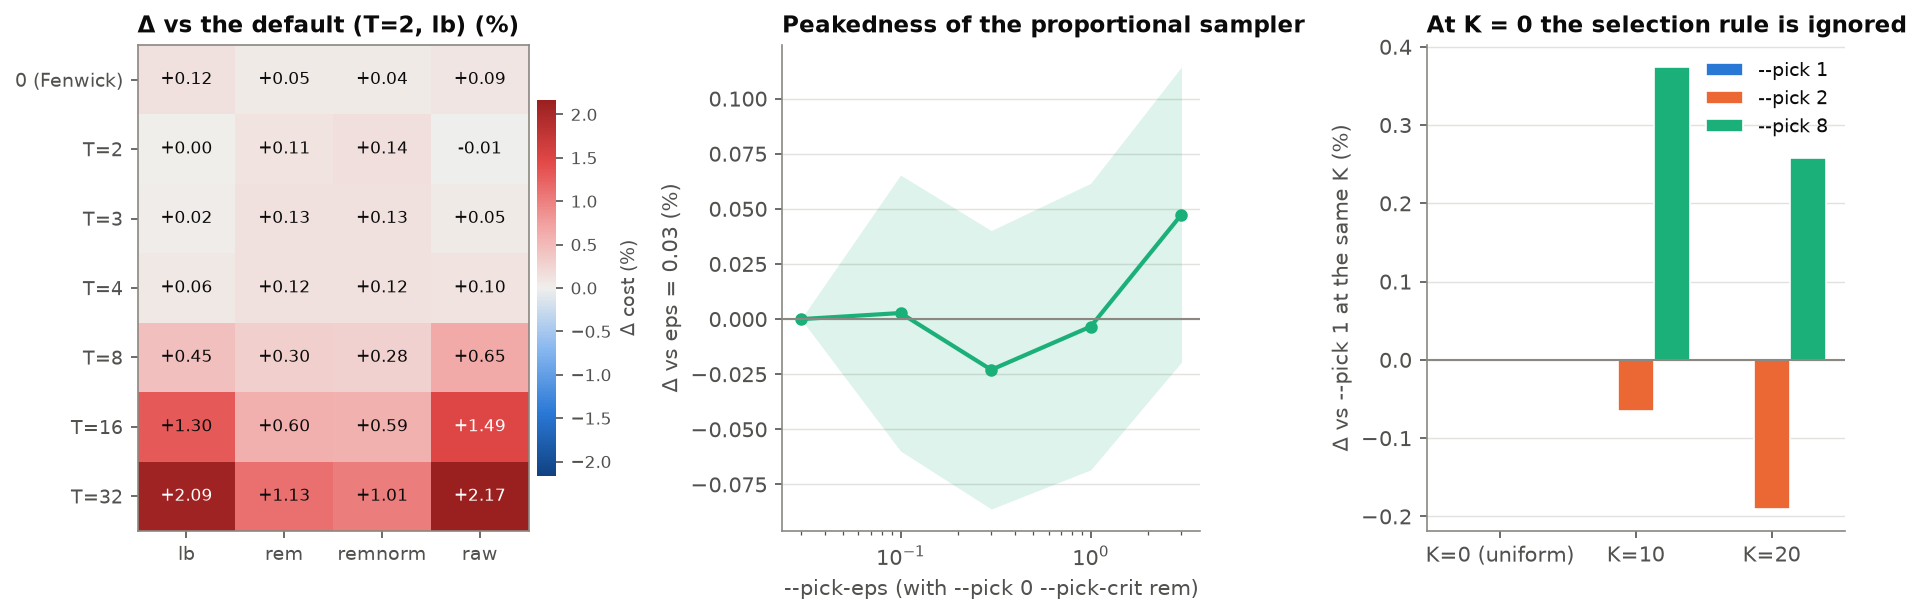
\includegraphics[width=\linewidth,height=0.74\textheight,keepaspectratio]{figures/pick.png}
  \caption{Left: tournament size against regret criterion. Middle: peakedness of the proportional sampler. Right: \texttt{-{}-pick} crossed with \texttt{-{}-sa-knn}; the flat $K=0$ group is the silent fallback.}
\end{figure}

{\small\begin{longtable}{llrrrr}
\caption{Tournament size against regret criterion, paired against the default $T=2$ with \texttt{lb}.}\\
\toprule
\textbf{\texttt{-{}-pick}} & \textbf{\texttt{-{}-pick-crit}} & \textbf{mean cost} & \textbf{$\Delta$ (\%)} & \textbf{95\,\% CI} & \textbf{win/loss} \\
\midrule
\endfirsthead
\toprule
\textbf{\texttt{-{}-pick}} & \textbf{\texttt{-{}-pick-crit}} & \textbf{mean cost} & \textbf{$\Delta$ (\%)} & \textbf{95\,\% CI} & \textbf{win/loss} \\
\midrule
\endhead
  1 (uniform) & -- & 16.07184 & \textbf{+0.191} & [+0.120,\;+0.262] & 452/544 \\
  0 (Fenwick) & \texttt{lb} & 16.06037 & \textbf{+0.119} & [+0.048,\;+0.190] & 466/531 \\
  0 (Fenwick) & \texttt{rem} & 16.04919 & +0.050 & [-0.018,\;+0.117] & 484/513 \\
  0 (Fenwick) & \texttt{remnorm} & 16.04781 & +0.041 & [-0.027,\;+0.109] & 494/503 \\
  0 (Fenwick) & \texttt{raw} & 16.05556 & +0.089 & [+0.018,\;+0.161] & 479/517 \\
  2 & \texttt{lb} & 16.04122 & +0.000 & [+0.000,\;+0.000] & 0/0 \\
  2 & \texttt{rem} & 16.05952 & +0.114 & [+0.045,\;+0.183] & 476/520 \\
  2 & \texttt{remnorm} & 16.06325 & \textbf{+0.137} & [+0.068,\;+0.206] & 439/554 \\
  2 & \texttt{raw} & 16.03902 & -0.014 & [-0.085,\;+0.058] & 508/488 \\
  3 & \texttt{lb} & 16.04460 & +0.021 & [-0.046,\;+0.088] & 492/506 \\
  3 & \texttt{rem} & 16.06149 & \textbf{+0.126} & [+0.058,\;+0.195] & 468/531 \\
  3 & \texttt{remnorm} & 16.06162 & +0.127 & [+0.061,\;+0.194] & 472/526 \\
  3 & \texttt{raw} & 16.04923 & +0.050 & [-0.019,\;+0.119] & 498/499 \\
  4 & \texttt{lb} & 16.05119 & +0.062 & [-0.011,\;+0.135] & 473/525 \\
  4 & \texttt{rem} & 16.06065 & \textbf{+0.121} & [+0.053,\;+0.189] & 448/551 \\
  4 & \texttt{remnorm} & 16.06075 & \textbf{+0.122} & [+0.051,\;+0.192] & 462/534 \\
  4 & \texttt{raw} & 16.05774 & \textbf{+0.103} & [+0.034,\;+0.172] & 465/531 \\
  8 & \texttt{lb} & 16.11339 & \textbf{+0.450} & [+0.380,\;+0.520] & 349/645 \\
  8 & \texttt{rem} & 16.08857 & \textbf{+0.295} & [+0.224,\;+0.367] & 390/607 \\
  8 & \texttt{remnorm} & 16.08641 & \textbf{+0.282} & [+0.213,\;+0.350] & 400/598 \\
  8 & \texttt{raw} & 16.14589 & \textbf{+0.653} & [+0.580,\;+0.725] & 286/709 \\
  16 & \texttt{lb} & 16.24928 & \textbf{+1.297} & [+1.221,\;+1.373] & 123/866 \\
  16 & \texttt{rem} & 16.13780 & \textbf{+0.602} & [+0.529,\;+0.675] & 321/677 \\
  16 & \texttt{remnorm} & 16.13574 & \textbf{+0.589} & [+0.519,\;+0.659] & 298/701 \\
  16 & \texttt{raw} & 16.27994 & \textbf{+1.488} & [+1.412,\;+1.565] & 86/906 \\
  32 & \texttt{lb} & 16.37717 & \textbf{+2.094} & [+2.013,\;+2.175] & 30/955 \\
  32 & \texttt{rem} & 16.22282 & \textbf{+1.132} & [+1.054,\;+1.210] & 171/826 \\
  32 & \texttt{remnorm} & 16.20300 & \textbf{+1.009} & [+0.936,\;+1.081] & 187/811 \\
  32 & \texttt{raw} & 16.38922 & \textbf{+2.169} & [+2.087,\;+2.252] & 20/964 \\
\bottomrule
\end{longtable}}

\begin{table}[H]\centering\small
\begin{tabular}{rrrrrr}
\toprule
\textbf{\texttt{-{}-sa-knn}} & \textbf{\texttt{-{}-pick}} & \textbf{mean cost} & \textbf{$\Delta$ (\%)} & \textbf{95\,\% CI} & \textbf{win/loss} \\
\midrule
  0 & 1 & 16.40787 & +0.000 & [+0.000,\;+0.000] & 0/0 \\
  10 & 1 & 16.09302 & +0.000 & [+0.000,\;+0.000] & 0/0 \\
  20 & 1 & 16.07184 & +0.000 & [+0.000,\;+0.000] & 0/0 \\
  0 & 2 & 16.40787 & +0.000 & [+0.000,\;+0.000] & 0/0 \\
  10 & 2 & 16.08260 & -0.065 & [-0.125,\;-0.005] & 514/470 \\
  20 & 2 & 16.04122 & \textbf{-0.190} & [-0.261,\;-0.120] & 544/452 \\
  0 & 8 & 16.40787 & +0.000 & [+0.000,\;+0.000] & 0/0 \\
  10 & 8 & 16.15324 & \textbf{+0.374} & [+0.310,\;+0.438] & 346/651 \\
  20 & 8 & 16.11339 & \textbf{+0.259} & [+0.187,\;+0.330] & 394/603 \\
\bottomrule
\end{tabular}
\caption{\texttt{-{}-pick} crossed with \texttt{-{}-sa-knn}, paired against \texttt{-{}-pick 1} at the same $K$. The $K=0$ rows are exactly zero because \texttt{cw.c:1676} forces uniform selection there --- while the run header still prints the requested rule.}
\end{table}

\textbf{Reading.} The prediction was wrong. At $n=100$ with $10^5$ steps the
entire grid --- every tournament size, every criterion, and the Fenwick sampler
--- sits inside $\pm 0.08\,\%$ of the default. The regret machinery is
measurable in the code but not in the result: whatever it saves in draw quality
it appears to give back in draw cost. It is only at $T \ge 16$ with \texttt{lb}
or \texttt{raw} that the choice starts to hurt, from over-concentrating on a few
vertices. The one solid finding here is the silent fallback at $K=0$: the header
reports a rule the code is not using.


\section{Biasing the second vertex}\label{sec:select}

\textbf{What it controls.} Section~\ref{sec:pick} is about choosing the vertex
$u$ to move. These three knobs are about the \emph{partner} $v$, and about where
$u$ is put once chosen.
\begin{itemize}\itemsep2pt
  \item \texttt{-{}-vrank T} --- the kNN lists are stored sorted by distance, so
        drawing the index as the \emph{minimum of $T$ uniform draws} biases
        towards the nearer neighbours at no memory access at all. $T=1$ is the
        plain uniform draw.
  \item \texttt{-{}-pick2 T} --- a tournament of size $T$ among candidate
        partners, keeping the one of largest regret. Unlike \texttt{-{}-vrank}
        this one costs a memory read per candidate.
  \item \texttt{-{}-reloc-side long} --- relocate breaks the \emph{longer} of
        the two edges adjacent to $v$ instead of flipping a coin, which
        maximises the $-d(v,q)$ term of the insertion cost. Two reads, no
        randomness.
\end{itemize}

\textbf{The question.} \texttt{-{}-vrank} is claimed to be \emph{coupled} with
\texttt{-{}-sa-knn}: a longer candidate list gives the reach, the rank bias
restores the concentration, and either one alone is supposed to hurt. That is
only testable on the grid, so the grid is what is run.

\begin{figure}[H]\centering
  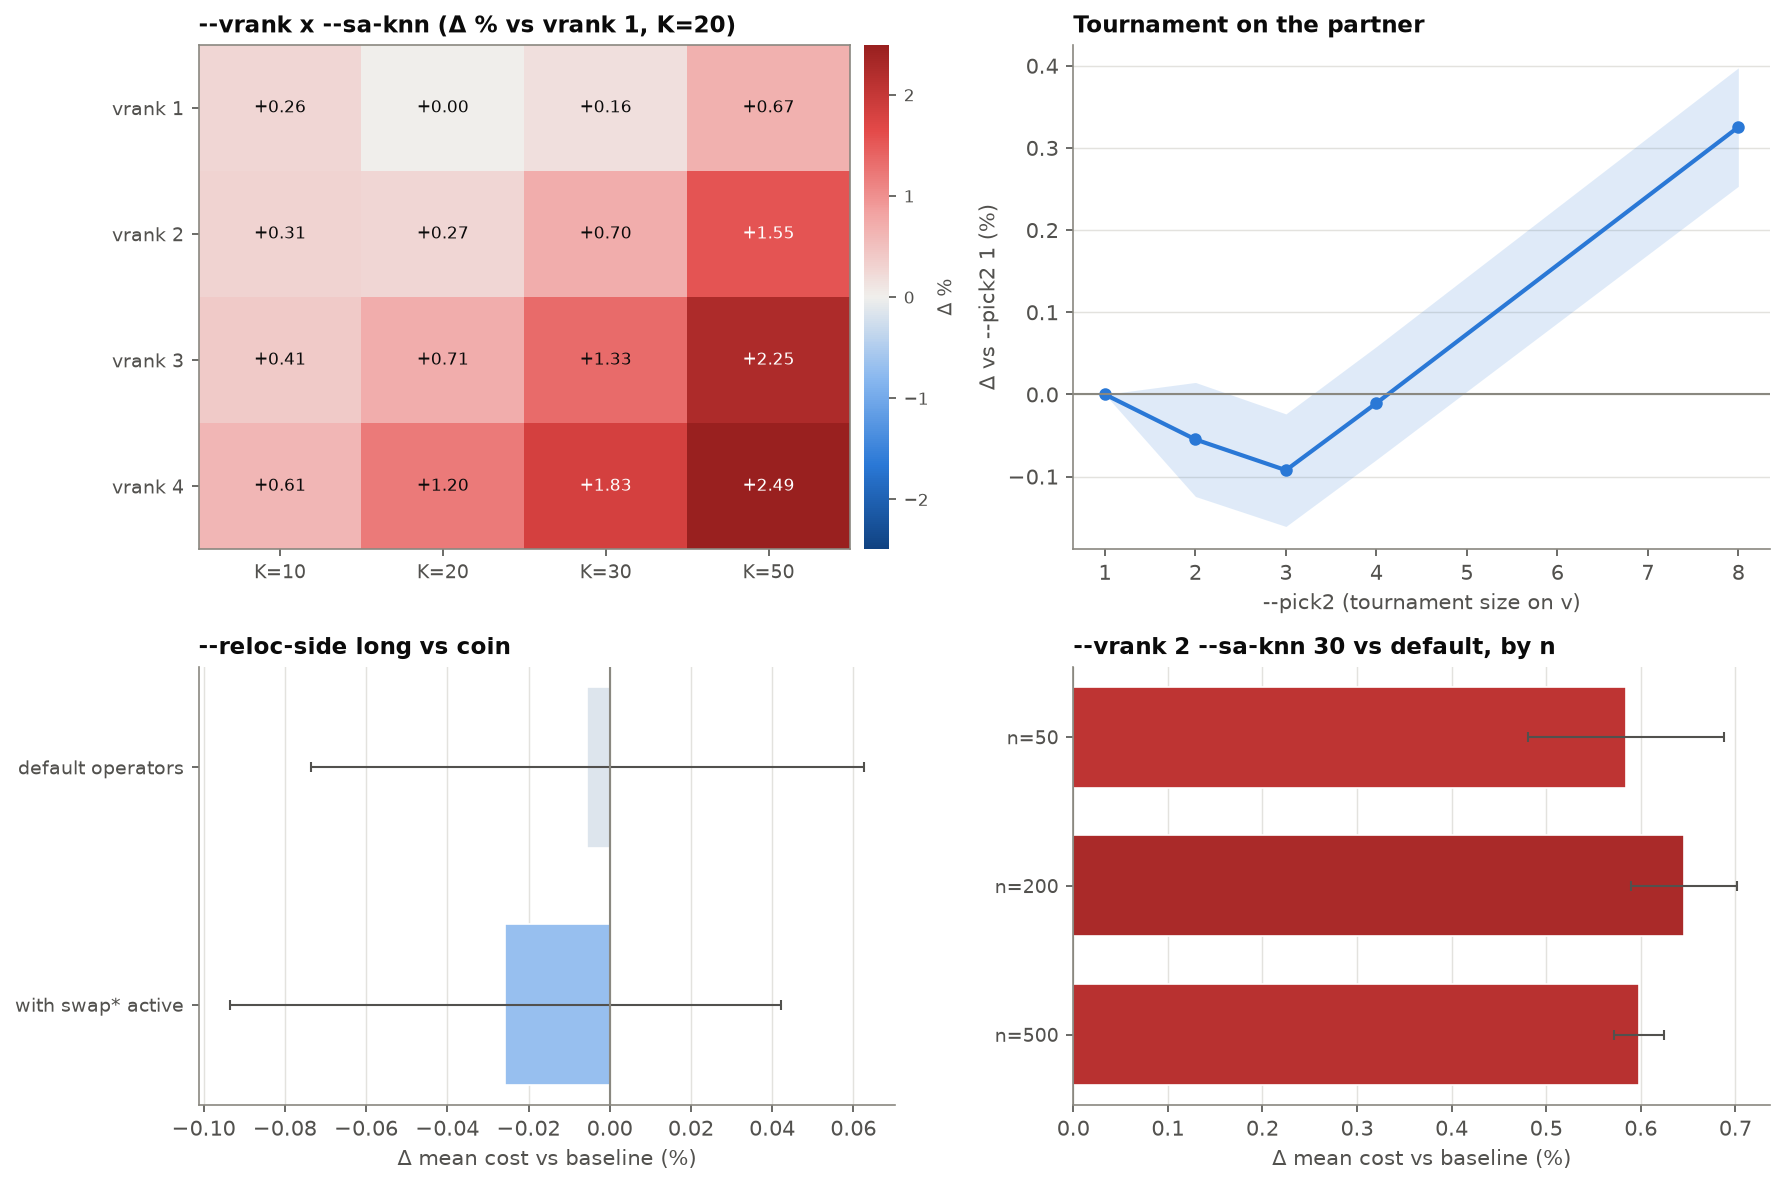
\includegraphics[width=\linewidth,height=0.74\textheight,keepaspectratio]{figures/select.png}
  \caption{Top left: the \texttt{-{}-vrank}/\texttt{-{}-sa-knn} grid, the coupling claim. Top right: tournament size on the partner. Bottom left: the relocate insertion side. Bottom right: the recommended \texttt{-{}-vrank 2 -{}-sa-knn 30} pair across dimension.}
\end{figure}

{\small\begin{longtable}{rrrrrr}
\caption{The full \texttt{-{}-vrank} $\times$ \texttt{-{}-sa-knn} grid, paired against \texttt{vrank 1, K=20} (the default).}\\
\toprule
\textbf{\texttt{-{}-vrank}} & \textbf{\texttt{-{}-sa-knn}} & \textbf{mean cost} & \textbf{$\Delta$ (\%)} & \textbf{95\,\% CI} & \textbf{win/loss} \\
\midrule
\endfirsthead
\toprule
\textbf{\texttt{-{}-vrank}} & \textbf{\texttt{-{}-sa-knn}} & \textbf{mean cost} & \textbf{$\Delta$ (\%)} & \textbf{95\,\% CI} & \textbf{win/loss} \\
\midrule
\endhead
  1 & 10 & 16.08260 & \textbf{+0.258} & [+0.190,\;+0.326] & 406/590 \\
  1 & 20 & 16.04122 & +0.000 & [+0.000,\;+0.000] & 0/0 \\
  1 & 30 & 16.06646 & \textbf{+0.157} & [+0.079,\;+0.236] & 434/558 \\
  1 & 50 & 16.14911 & \textbf{+0.673} & [+0.588,\;+0.757] & 292/696 \\
  2 & 10 & 16.09055 & \textbf{+0.307} & [+0.242,\;+0.373] & 395/601 \\
  2 & 20 & 16.08441 & \textbf{+0.269} & [+0.194,\;+0.344] & 413/584 \\
  2 & 30 & 16.15421 & \textbf{+0.704} & [+0.622,\;+0.787] & 291/701 \\
  2 & 50 & 16.29032 & \textbf{+1.553} & [+1.470,\;+1.636] & 100/884 \\
  3 & 10 & 16.10678 & \textbf{+0.409} & [+0.337,\;+0.481] & 360/633 \\
  3 & 20 & 16.15477 & \textbf{+0.708} & [+0.631,\;+0.784] & 251/737 \\
  3 & 30 & 16.25393 & \textbf{+1.326} & [+1.246,\;+1.406] & 139/851 \\
  3 & 50 & 16.40241 & \textbf{+2.252} & [+2.167,\;+2.336] & 16/964 \\
  4 & 10 & 16.13852 & \textbf{+0.607} & [+0.535,\;+0.678] & 284/709 \\
  4 & 20 & 16.23370 & \textbf{+1.200} & [+1.121,\;+1.279] & 153/836 \\
  4 & 30 & 16.33483 & \textbf{+1.830} & [+1.750,\;+1.910] & 53/930 \\
  4 & 50 & 16.44123 & \textbf{+2.494} & [+2.406,\;+2.581] & 2/977 \\
\bottomrule
\end{longtable}}

\begin{table}[H]\centering\small
\begin{tabular}{lrrrrr}
\toprule
\textbf{context} & \textbf{coin} & \textbf{long} & \textbf{$\Delta$ (\%)} & \textbf{95\,\% CI} & \textbf{win/loss} \\
\midrule
  default operators & 16.04122 & 16.04034 & -0.006 & [-0.074,\;+0.063] & 496/496 \\
  with swap* active & 15.90965 & 15.90557 & -0.026 & [-0.093,\;+0.042] & 529/470 \\
\bottomrule
\end{tabular}
\caption{The relocate insertion side, with and without swap* active.}
\end{table}

\begin{table}[H]\centering\small
\begin{tabular}{rrrrrr}
\toprule
\textbf{$n$} & \textbf{default} & \textbf{vrank 2, K=30} & \textbf{$\Delta$ (\%)} & \textbf{95\,\% CI} & \textbf{win/loss} \\
\midrule
  50 & 10.53078 & 10.59232 & \textbf{+0.584} & [+0.481,\;+0.688] & 314/649 \\
  200 & 22.91368 & 23.06157 & \textbf{+0.645} & [+0.589,\;+0.702] & 232/765 \\
  500 & 39.05297 & 39.28644 & \textbf{+0.598} & [+0.571,\;+0.624] & 75/925 \\
\bottomrule
\end{tabular}
\caption{The rank bias with the longer candidate list, across dimension.}
\end{table}

\textbf{Reading.} The coupling claim does not reproduce here, and the heat map
is unusually unambiguous about it: the best cell of the whole grid is the
default corner, every increase in \texttt{-{}-vrank} makes things worse at every
$K$, and the effect compounds --- the supposed winning combination, a longer
list with a stronger rank bias, is among the worst cells tried. The most likely
explanation is that the claim was made against a construction that shares one
$K=30$ neighbour list between the savings and the annealing, whereas here the
savings are exact for $n \le 1500$ and the annealing builds its own list. Those
are not the same baseline, and this sweep cannot settle which is right for the
other one --- only that on this code, at this budget, the rank bias costs.

\texttt{-{}-pick2} is the mild surprise: a tournament of 3 on the partner is a
small but genuine improvement, which makes it the only selection bias in this
document that survives while costing a memory read per candidate. It is worth
about a tenth of what swap* is worth, and the curve is flat enough between 2 and
4 that the exact size does not matter. The relocate insertion side moves in the
right direction with and without swap* active, but neither interval excludes
zero: on this evidence it is free rather than useful, and it is left off.


\section{Racing between restarts, and interleaving}\label{sec:race}

\textbf{What it controls.} Section~\ref{sec:restarts} spends the budget equally
over the restarts. \texttt{-{}-race M} spends it unequally instead: at
\texttt{-{}-race-at} of its own budget (a quarter by default) a start is
compared with the best \emph{finished} start \emph{at the same point of its
trajectory} --- same temperature, which is what makes the comparison fair --- and
abandoned if it is worse by a relative margin $M$. Its unspent steps lengthen the
schedules of the starts that follow, and whatever is left at the end is spent
polishing the best solution found. The total step budget never changes; only its
allocation does.

\texttt{-{}-pair} is a different kind of knob: two starts are advanced
alternately in the same loop so that one's memory latency overlaps with the
other's arithmetic. Each chain owns its solution, its incremental buffers and its
random stream, so without \texttt{-{}-race} the trajectories are identical bit
for bit and only the clock may move. That makes it a self-checking row in the
table below: if the cost column is not flat, something is wrong.

\textbf{The question.} Every run in this section holds
$\texttt{restarts} \times \texttt{sa-steps}$ constant, because a racing gain at
unequal budget would be meaningless.

\begin{figure}[H]\centering
  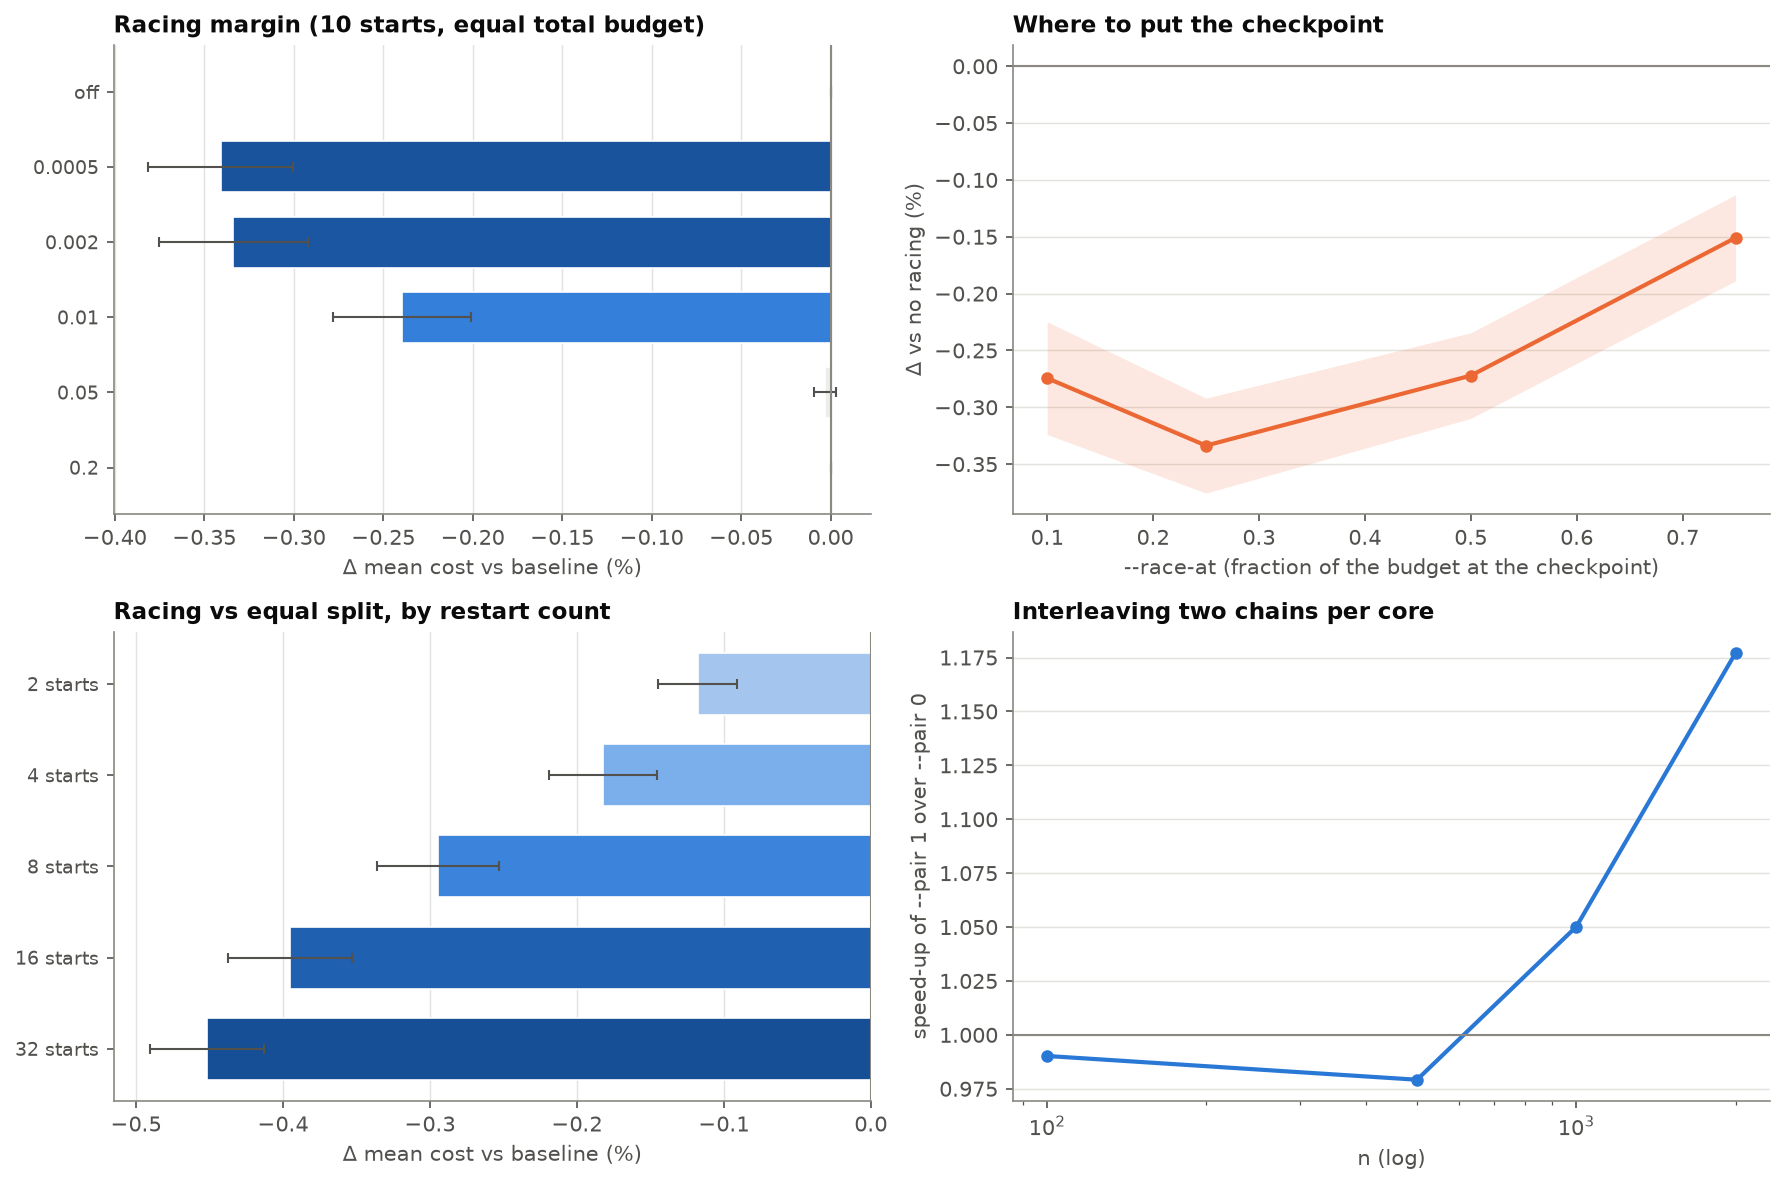
\includegraphics[width=\linewidth,height=0.74\textheight,keepaspectratio]{figures/race.png}
  \caption{Top: the racing margin and the checkpoint position, both at equal total budget. Bottom left: racing against an equal split as the number of starts grows. Bottom right: the interleaving speed-up, which is a timing result only --- the costs are identical.}
\end{figure}

\begin{table}[H]\centering\small
\begin{tabular}{rrrrr}
\toprule
\textbf{margin} & \textbf{mean cost} & \textbf{$\Delta$ (\%)} & \textbf{95\,\% CI} & \textbf{win/loss} \\
\midrule
  off & 15.88401 & +0.000 & [+0.000,\;+0.000] & 0/0 \\
  0.0005 & 15.82986 & \textbf{-0.341} & [-0.381,\;-0.300] & 658/261 \\
  0.002 & 15.83100 & \textbf{-0.334} & [-0.375,\;-0.292] & 646/265 \\
  0.01 & 15.84598 & \textbf{-0.239} & [-0.278,\;-0.201] & 560/263 \\
  0.05 & 15.88352 & -0.003 & [-0.009,\;+0.003] & 29/18 \\
  0.2 & 15.88401 & +0.000 & [+0.000,\;+0.000] & 0/0 \\
\bottomrule
\end{tabular}
\caption{Racing margin, 10 starts at equal total budget.}
\end{table}

\begin{table}[H]\centering\small
\begin{tabular}{rrrrr}
\toprule
\textbf{\texttt{-{}-race-at}} & \textbf{mean cost} & \textbf{$\Delta$ (\%)} & \textbf{95\,\% CI} & \textbf{win/loss} \\
\midrule
  0.1 & 15.84042 & \textbf{-0.274} & [-0.324,\;-0.225] & 605/322 \\
  0.25 & 15.83100 & \textbf{-0.334} & [-0.375,\;-0.292] & 646/265 \\
  0.5 & 15.84078 & \textbf{-0.272} & [-0.310,\;-0.234] & 640/266 \\
  0.75 & 15.86004 & \textbf{-0.151} & [-0.189,\;-0.113] & 563/326 \\
\bottomrule
\end{tabular}
\caption{Position of the checkpoint, at margin 0.002.}
\end{table}

\begin{table}[H]\centering\small
\begin{tabular}{rrrrrr}
\toprule
\textbf{starts} & \textbf{equal split} & \textbf{racing} & \textbf{$\Delta$ (\%)} & \textbf{95\,\% CI} & \textbf{win/loss} \\
\midrule
  2 & 15.88342 & 15.86471 & \textbf{-0.118} & [-0.145,\;-0.091] & 226/58 \\
  4 & 15.87705 & 15.84812 & \textbf{-0.182} & [-0.219,\;-0.145] & 479/202 \\
  8 & 15.88281 & 15.83601 & \textbf{-0.295} & [-0.336,\;-0.253] & 589/290 \\
  16 & 15.88591 & 15.82312 & \textbf{-0.395} & [-0.437,\;-0.353] & 726/233 \\
  32 & 15.89661 & 15.82481 & \textbf{-0.452} & [-0.491,\;-0.413] & 761/218 \\
\bottomrule
\end{tabular}
\caption{Racing against an equal split, holding $\texttt{restarts} \times \texttt{sa-steps}$ constant.}
\end{table}

\begin{table}[H]\centering\small
\begin{tabular}{rrrlrrr}
\toprule
\textbf{$n$} & \textbf{\texttt{-{}-pair 0}} & \textbf{\texttt{-{}-pair 1}} & \textbf{identical} & \textbf{wall 0} & \textbf{wall 1} & \textbf{speed-up} \\
\midrule
  100 & 15.88281 & 15.88281 & yes & 1.62s & 1.63s & 0.99x \\
  500 & 39.01207 & 39.01207 & yes & 2.92s & 2.98s & 0.98x \\
  1000 & 45.64863 & 45.64863 & yes & 6.36s & 6.06s & 1.05x \\
  2000 & 80.05502 & 80.05502 & yes & 6.26s & 5.32s & 1.18x \\
\bottomrule
\end{tabular}
\caption{Interleaving. The \emph{identical} column is the check that this is an engineering change and not an algorithmic one: the two costs must agree exactly.}
\end{table}

\textbf{Reading.} Racing needs starts to race: with two it has almost nothing to
redistribute, and the gain grows steadily with the restart count. It is the
second largest effect in this document after swap*, and it costs nothing --- the
budget is the same, only its allocation changes.

The margin behaves monotonically over the range tried, which is worth noting
because it was not the expectation: the tightest margin is the best one, and
loosening it only ever gives ground back. By $0.05$ almost no start is ever
behind by that much at the checkpoint, so the setting is indistinguishable from
\texttt{off}, and by $0.2$ it is exactly \texttt{off}. There was reason to expect
the other failure mode as well --- a margin so tight that good starts are killed
on noise --- and this sweep does not reach it, so the bottom of the useful range
is still unmeasured. The checkpoint position matters much less than the margin;
anything from a tenth to half of the budget is within noise of the default
quarter, and only pushing it out to three quarters clearly hurts, by which point
most of the budget the racing was meant to reclaim has already been spent.

\texttt{-{}-pair} does exactly what it claims. The \emph{identical} column reads
\texttt{yes} on every row --- the interleaved chains reproduce the sequential
trajectories exactly --- and the speed-up appears only once the state of one
chain stops fitting in the low-level caches: slightly negative at $n \le 500$,
where the bookkeeping is not paid back, and clearly positive from $n = 1000$.
That is a smaller effect than the $1.42\times$ reported for the implementation
this was ported from; the shape of the curve is the same, so the difference is
most likely the cache hierarchy of the machine rather than the technique.


\section{Annealing schedule}\label{sec:temp}

\textbf{What it controls.} The initial temperature $T_0$ is not given directly:
\texttt{calibrate\_T0} samples worsening moves on the actual instance and solves
for the $T_0$ whose acceptance probability matches \texttt{-{}-t-accept} (default
$0.001$, i.e.\ $0.1\,\%$ of worsening moves accepted at the start). The
temperature then decays geometrically to $T_0 \cdot 10^{-D}$ over the whole run,
with $D =$ \texttt{-{}-t-decades} (default 2). Together they fix both ends of the
schedule; \texttt{-{}-t0} and \texttt{-{}-tend} override the calibration.

\begin{figure}[H]\centering
  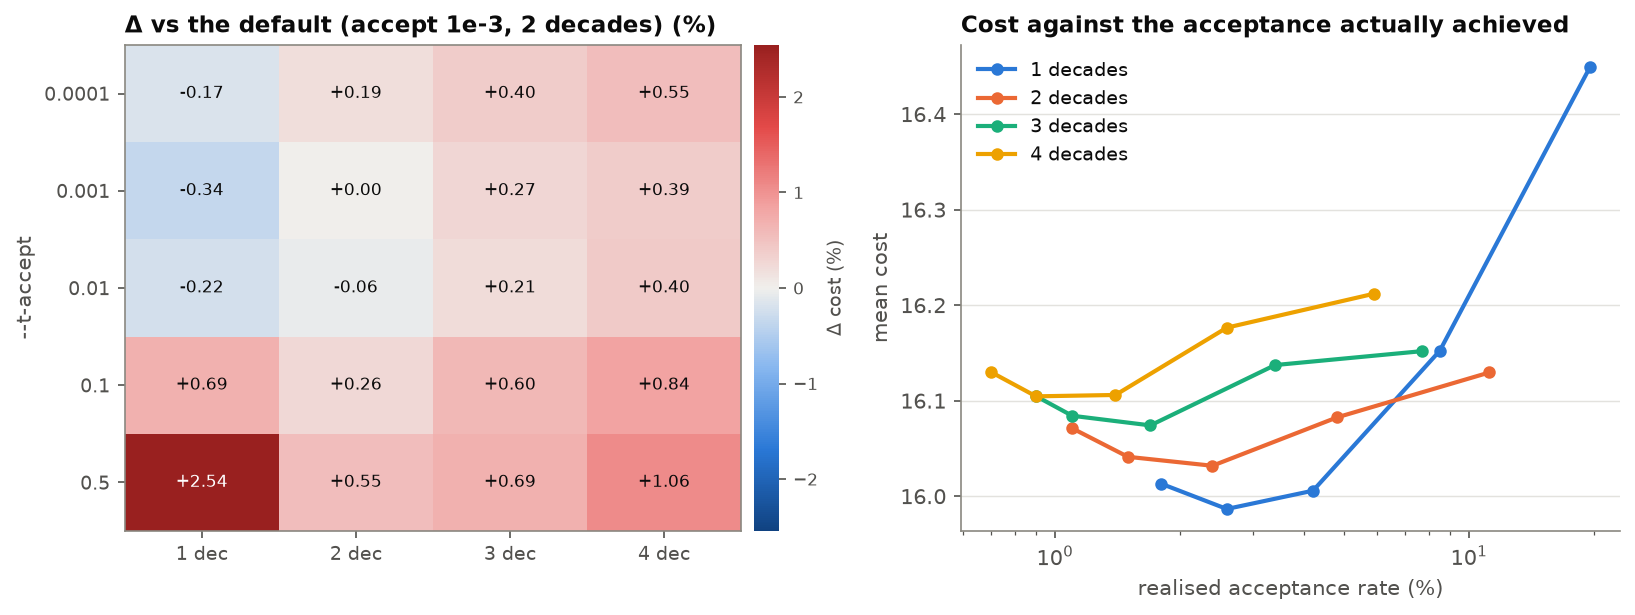
\includegraphics[width=\linewidth,height=0.74\textheight,keepaspectratio]{figures/temp.png}
  \caption{Left: the full \texttt{-{}-t-accept} $\times$ \texttt{-{}-t-decades} grid. Right: the same runs plotted against the acceptance rate they actually realised.}
\end{figure}

{\small\begin{longtable}{rrrrrrr}
\caption{Annealing schedule, paired against the default ($\texttt{t-accept}=10^{-3}$, 2 decades).}\\
\toprule
\textbf{\texttt{-{}-t-accept}} & \textbf{\texttt{-{}-t-decades}} & \textbf{mean cost} & \textbf{accept.\ (\%)} & \textbf{$\Delta$ (\%)} & \textbf{95\,\% CI} & \textbf{win/loss} \\
\midrule
\endfirsthead
\toprule
\textbf{\texttt{-{}-t-accept}} & \textbf{\texttt{-{}-t-decades}} & \textbf{mean cost} & \textbf{accept.\ (\%)} & \textbf{$\Delta$ (\%)} & \textbf{95\,\% CI} & \textbf{win/loss} \\
\midrule
\endhead
  0.0001 & 1 & 16.01326 & 1.80 & \textbf{-0.174} & [-0.243,\;-0.105] & 558/441 \\
  0.0001 & 2 & 16.07112 & 1.10 & \textbf{+0.186} & [+0.119,\;+0.253] & 447/550 \\
  0.0001 & 3 & 16.10473 & 0.90 & \textbf{+0.396} & [+0.328,\;+0.464] & 386/609 \\
  0.0001 & 4 & 16.13003 & 0.70 & \textbf{+0.554} & [+0.486,\;+0.621] & 299/694 \\
  0.001 & 1 & 15.98661 & 2.60 & \textbf{-0.340} & [-0.413,\;-0.268] & 610/384 \\
  0.001 & 2 & 16.04122 & 1.50 & +0.000 & [+0.000,\;+0.000] & 0/0 \\
  0.001 & 3 & 16.08422 & 1.10 & \textbf{+0.268} & [+0.201,\;+0.335] & 401/590 \\
  0.001 & 4 & 16.10453 & 0.90 & \textbf{+0.395} & [+0.324,\;+0.465] & 347/648 \\
  0.01 & 1 & 16.00576 & 4.20 & \textbf{-0.221} & [-0.304,\;-0.138] & 558/434 \\
  0.01 & 2 & 16.03185 & 2.40 & -0.058 & [-0.140,\;+0.023] & 505/492 \\
  0.01 & 3 & 16.07411 & 1.70 & \textbf{+0.205} & [+0.129,\;+0.281] & 418/574 \\
  0.01 & 4 & 16.10597 & 1.40 & \textbf{+0.404} & [+0.329,\;+0.478] & 354/635 \\
  0.1 & 1 & 16.15225 & 8.50 & \textbf{+0.692} & [+0.604,\;+0.781] & 299/689 \\
  0.1 & 2 & 16.08249 & 4.80 & \textbf{+0.257} & [+0.163,\;+0.352] & 409/583 \\
  0.1 & 3 & 16.13728 & 3.40 & \textbf{+0.599} & [+0.506,\;+0.692] & 311/677 \\
  0.1 & 4 & 16.17643 & 2.60 & \textbf{+0.843} & [+0.752,\;+0.933] & 270/718 \\
  0.5 & 1 & 16.44932 & 19.60 & \textbf{+2.544} & [+2.456,\;+2.632] & 0/979 \\
  0.5 & 2 & 16.12953 & 11.20 & \textbf{+0.551} & [+0.459,\;+0.642] & 308/679 \\
  0.5 & 3 & 16.15184 & 7.70 & \textbf{+0.690} & [+0.593,\;+0.786] & 301/689 \\
  0.5 & 4 & 16.21200 & 5.90 & \textbf{+1.065} & [+0.976,\;+1.153] & 207/780 \\
\bottomrule
\end{longtable}}

\textbf{Reading.} This is the largest effect in the whole sweep. Narrowing the
temperature range to a single decade is worth about $-0.37\,\%$ --- more than
every operator, neighbourhood and selection setting combined. The interpretation
is that at $10^5$ steps the default schedule spends too long at temperatures so
low that nothing is accepted: the run is effectively over before the step budget
is. Fewer decades keeps the search alive for more of the run. This also implies
the right number of decades depends on the budget, so it should be re-checked
when \texttt{-{}-sa-steps} changes substantially.


\section{Construction quality}\label{sec:construct}

\textbf{What it controls.} Three separate things about the Clarke \& Wright
stage. The savings formula
$s(i,j) = d_{0i} + d_{0j} - \lambda\,d_{ij} + \mu\,|d_{0i}-d_{0j}|$ has two shape
parameters: \texttt{-{}-lambda} sets how much weight the direct link between two
customers carries against their two depot legs (the classical generalisation of
Clarke \& Wright, $\lambda > 1$ favouring longer, less radial routes), and
\texttt{-{}-mu} adds an asymmetry term penalising the merge of two customers at
very different distances from the depot. \texttt{-{}-knn K} truncates the savings
list to each customer's $K$ nearest neighbours instead of all $O(n^2)$ pairs
(\texttt{-{}-exact} forces the full list; the default is exact for
$n \le 1500$). \texttt{-{}-2opt} runs an intra-route 2-opt pass after the
construction.

\textbf{The question.} Every one of these improves or degrades the \emph{starting}
solution. The interesting question is whether that survives the annealing, so each
grid is run twice: with \texttt{-{}-no-sa} and with the full budget.

{\small\begin{longtable}{rrrrrr}
\caption{Savings parameters, construction only, paired against $\lambda=1$, $\mu=0$.}\\
\toprule
\textbf{$\lambda$} & \textbf{$\mu$} & \textbf{mean cost} & \textbf{$\Delta$ (\%)} & \textbf{95\,\% CI} & \textbf{win/loss} \\
\midrule
\endfirsthead
\toprule
\textbf{$\lambda$} & \textbf{$\mu$} & \textbf{mean cost} & \textbf{$\Delta$ (\%)} & \textbf{95\,\% CI} & \textbf{win/loss} \\
\midrule
\endhead
  0.6 & 0 & 17.04835 & \textbf{+3.639} & [+3.496,\;+3.782] & 42/958 \\
  0.6 & 0.2 & 17.07377 & \textbf{+3.794} & [+3.657,\;+3.931] & 34/966 \\
  0.6 & 0.5 & 17.08990 & \textbf{+3.892} & [+3.753,\;+4.031] & 39/961 \\
  0.6 & 1 & 17.13273 & \textbf{+4.152} & [+3.996,\;+4.308] & 52/948 \\
  0.8 & 0 & 16.65490 & \textbf{+1.247} & [+1.140,\;+1.354] & 207/793 \\
  0.8 & 0.2 & 16.72637 & \textbf{+1.682} & [+1.571,\;+1.792] & 142/858 \\
  0.8 & 0.5 & 16.81977 & \textbf{+2.250} & [+2.126,\;+2.374] & 135/865 \\
  0.8 & 1 & 17.00364 & \textbf{+3.367} & [+3.218,\;+3.517] & 88/912 \\
  1 & 0 & 16.44971 & +0.000 & [+0.000,\;+0.000] & 0/0 \\
  1 & 0.2 & 16.50233 & \textbf{+0.320} & [+0.228,\;+0.412] & 395/605 \\
  1 & 0.5 & 16.61998 & \textbf{+1.035} & [+0.919,\;+1.151] & 288/712 \\
  1 & 1 & 16.87703 & \textbf{+2.598} & [+2.461,\;+2.734] & 128/872 \\
  1.2 & 0 & 16.44126 & -0.051 & [-0.148,\;+0.045] & 514/485 \\
  1.2 & 0.2 & 16.37879 & \textbf{-0.431} & [-0.525,\;-0.337] & 574/402 \\
  1.2 & 0.5 & 16.47483 & \textbf{+0.153} & [+0.043,\;+0.262] & 459/541 \\
  1.2 & 1 & 16.76165 & \textbf{+1.896} & [+1.761,\;+2.031] & 206/794 \\
  1.4 & 0 & 16.50587 & \textbf{+0.341} & [+0.227,\;+0.456] & 425/575 \\
  1.4 & 0.2 & 16.38595 & \textbf{-0.388} & [-0.495,\;-0.281] & 598/402 \\
  1.4 & 0.5 & 16.38419 & \textbf{-0.398} & [-0.509,\;-0.288] & 584/416 \\
  1.4 & 1 & 16.66358 & \textbf{+1.300} & [+1.169,\;+1.431] & 266/734 \\
\bottomrule
\end{longtable}}

{\small\begin{longtable}{rrrrrr}
\caption{Savings parameters, after annealing, paired against $\lambda=1$, $\mu=0$.}\\
\toprule
\textbf{$\lambda$} & \textbf{$\mu$} & \textbf{mean cost} & \textbf{$\Delta$ (\%)} & \textbf{95\,\% CI} & \textbf{win/loss} \\
\midrule
\endfirsthead
\toprule
\textbf{$\lambda$} & \textbf{$\mu$} & \textbf{mean cost} & \textbf{$\Delta$ (\%)} & \textbf{95\,\% CI} & \textbf{win/loss} \\
\midrule
\endhead
  0.6 & 0 & 16.15903 & \textbf{+0.734} & [+0.620,\;+0.849] & 356/644 \\
  0.6 & 0.2 & 16.13108 & \textbf{+0.560} & [+0.453,\;+0.668] & 384/616 \\
  0.6 & 0.5 & 16.07839 & \textbf{+0.232} & [+0.134,\;+0.330] & 450/550 \\
  0.6 & 1 & 16.03138 & -0.061 & [-0.159,\;+0.036] & 522/478 \\
  0.8 & 0 & 16.08352 & \textbf{+0.264} & [+0.167,\;+0.360] & 449/551 \\
  0.8 & 0.2 & 16.07101 & \textbf{+0.186} & [+0.092,\;+0.279] & 465/534 \\
  0.8 & 0.5 & 16.05264 & +0.071 & [-0.026,\;+0.168] & 496/504 \\
  0.8 & 1 & 16.01874 & -0.140 & [-0.238,\;-0.043] & 522/478 \\
  1 & 0 & 16.04122 & +0.000 & [+0.000,\;+0.000] & 0/0 \\
  1 & 0.2 & 16.04110 & -0.001 & [-0.086,\;+0.084] & 505/495 \\
  1 & 0.5 & 16.03069 & -0.066 & [-0.158,\;+0.027] & 509/491 \\
  1 & 1 & 16.00930 & \textbf{-0.199} & [-0.293,\;-0.105] & 550/450 \\
  1.2 & 0 & 16.02356 & -0.110 & [-0.195,\;-0.025] & 524/475 \\
  1.2 & 0.2 & 16.01661 & -0.153 & [-0.238,\;-0.069] & 518/458 \\
  1.2 & 0.5 & 16.00808 & \textbf{-0.207} & [-0.298,\;-0.115] & 552/448 \\
  1.2 & 1 & 16.00301 & \textbf{-0.238} & [-0.334,\;-0.142] & 562/438 \\
  1.4 & 0 & 16.00966 & \textbf{-0.197} & [-0.288,\;-0.106] & 532/468 \\
  1.4 & 0.2 & 15.99763 & \textbf{-0.272} & [-0.362,\;-0.182] & 569/431 \\
  1.4 & 0.5 & 16.00097 & \textbf{-0.251} & [-0.343,\;-0.159] & 570/430 \\
  1.4 & 1 & 15.99932 & \textbf{-0.261} & [-0.354,\;-0.168] & 574/426 \\
\bottomrule
\end{longtable}}

\begin{figure}[H]\centering
  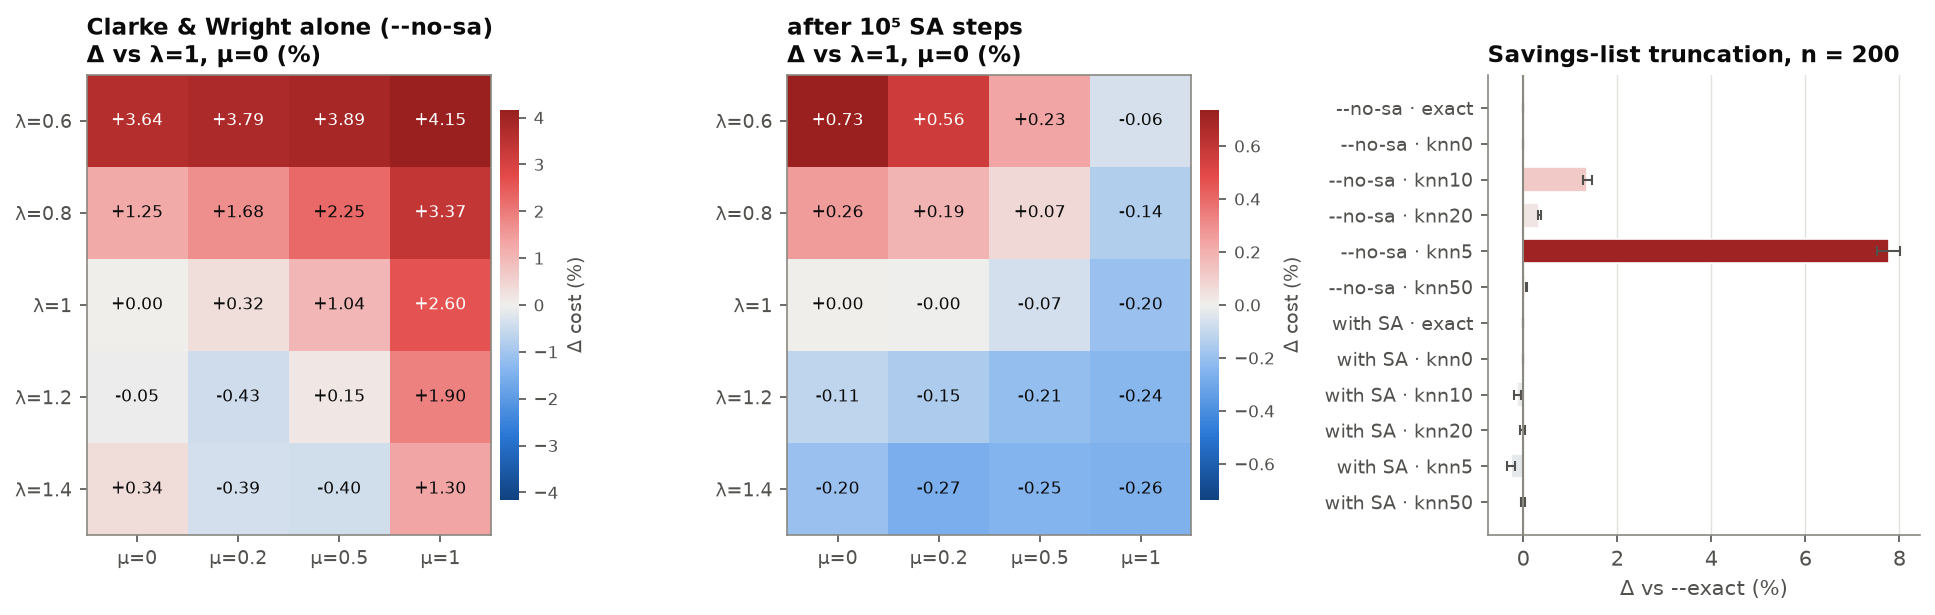
\includegraphics[width=\linewidth,height=0.74\textheight,keepaspectratio]{figures/construct.png}
  \caption{Left and middle: the same $\lambda \times \mu$ grid before and after annealing --- note the colour scales differ by an order of magnitude. Right: truncating the savings list, with and without annealing.}
\end{figure}

\begin{table}[H]\centering\small
\begin{tabular}{llrrrrr}
\toprule
\textbf{stage} & \textbf{variant} & \textbf{mean cost} & \textbf{$\Delta$ (\%)} & \textbf{95\,\% CI} & \textbf{win/loss} & \textbf{wall (s)} \\
\midrule
  \texttt{-{}-no-sa} & \texttt{exact} & 23.38509 & +0.000 & [+0.000,\;+0.000] & 0/0 & 0.02 \\
  \texttt{-{}-no-sa} & \texttt{knn0} & 23.38509 & +0.000 & [+0.000,\;+0.000] & 0/0 & 0.02 \\
  \texttt{-{}-no-sa} & \texttt{knn10} & 23.70418 & \textbf{+1.365} & [+1.272,\;+1.457] & 135/865 & 0.03 \\
  \texttt{-{}-no-sa} & \texttt{knn20} & 23.46603 & \textbf{+0.346} & [+0.304,\;+0.388] & 177/768 & 0.05 \\
  \texttt{-{}-no-sa} & \texttt{knn5} & 25.20278 & \textbf{+7.773} & [+7.526,\;+8.019] & 3/997 & 0.02 \\
  \texttt{-{}-no-sa} & \texttt{knn50} & 23.40135 & \textbf{+0.070} & [+0.054,\;+0.085] & 76/429 & 0.08 \\
  \texttt{with SA} & \texttt{exact} & 22.91368 & +0.000 & [+0.000,\;+0.000] & 0/0 & 0.43 \\
  \texttt{with SA} & \texttt{knn0} & 22.91368 & +0.000 & [+0.000,\;+0.000] & 0/0 & 0.47 \\
  \texttt{with SA} & \texttt{knn10} & 22.88483 & \textbf{-0.126} & [-0.196,\;-0.056] & 531/469 & 0.43 \\
  \texttt{with SA} & \texttt{knn20} & 22.91103 & -0.012 & [-0.069,\;+0.046] & 485/460 & 0.41 \\
  \texttt{with SA} & \texttt{knn5} & 22.85461 & \textbf{-0.258} & [-0.340,\;-0.176] & 576/424 & 0.46 \\
  \texttt{with SA} & \texttt{knn50} & 22.91303 & -0.003 & [-0.039,\;+0.034] & 257/248 & 0.50 \\
\bottomrule
\end{tabular}
\caption{Savings-list truncation at $n=200$, paired against \texttt{-{}-exact}. \texttt{knn0} is the automatic setting, which is exact at this size.}
\end{table}

\begin{table}[H]\centering\small
\begin{tabular}{lrrrrr}
\toprule
\textbf{stage} & \textbf{without \texttt{-{}-2opt}} & \textbf{with \texttt{-{}-2opt}} & \textbf{$\Delta$ (\%)} & \textbf{95\,\% CI} & \textbf{win/loss} \\
\midrule
  construction only & 16.44971 & 16.37485 & \textbf{-0.455} & [-0.476,\;-0.434] & 962/0 \\
  after annealing & 16.04122 & 16.03794 & -0.020 & [-0.087,\;+0.046] & 497/462 \\
\bottomrule
\end{tabular}
\caption{Intra-route 2-opt after the construction.}
\end{table}

\textbf{Reading.} Two opposite lessons. The savings \emph{shape} matters and
survives: $\lambda = 1.2$--$1.4$ with $\mu \approx 0.2$--$0.5$ is worth about
$-0.29\,\%$ after annealing, second only to the schedule. The savings
\emph{list}, by contrast, does not survive at all: truncating it to the 5 nearest
neighbours costs $+7.7\,\%$ on the raw construction and essentially nothing once
the annealing has run. That is a useful lever for large $n$, where
Section~\ref{sec:timing} showed the $O(n^2)$ list is the dominant cost --- the annealing repairs
what the truncation breaks. \texttt{-{}-2opt} is likewise absorbed: it improves
the construction and changes nothing afterwards.


\section{Do the knobs combine?}\label{sec:tuned}

\textbf{What is tested.} Tuning one knob at a time says nothing about tuning
several at once. These runs take three plausible changes, apply them
individually and together at equal SA budget, and compare against the stock
defaults. \texttt{all\_r8} additionally splits the same budget over 8 restarts.

\begin{figure}[H]\centering
  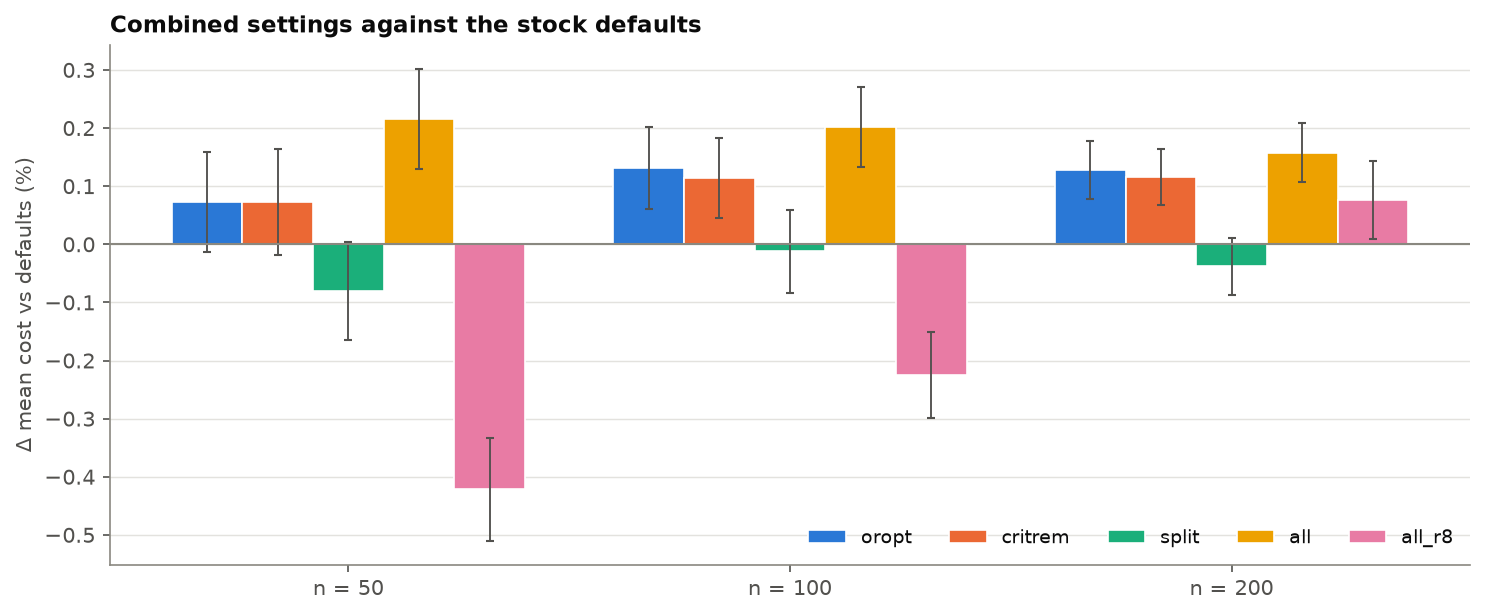
\includegraphics[width=\linewidth,height=0.74\textheight,keepaspectratio]{figures/tuned.png}
  \caption{Candidate combinations against the stock defaults at equal SA budget, with 95\,\% CIs.}
\end{figure}

{\small\begin{longtable}{rlrrrrr}
\caption{Combinations against the stock defaults.}\\
\toprule
\textbf{$n$} & \textbf{variant} & \textbf{mean cost} & \textbf{$\Delta$ (\%)} & \textbf{95\,\% CI} & \textbf{win/loss} & \textbf{wall (s)} \\
\midrule
\endfirsthead
\toprule
\textbf{$n$} & \textbf{variant} & \textbf{mean cost} & \textbf{$\Delta$ (\%)} & \textbf{95\,\% CI} & \textbf{win/loss} & \textbf{wall (s)} \\
\midrule
\endhead
  50 & or-opt enabled & 10.53841 & +0.073 & [-0.014,\;+0.159] & 455/471 & 0.37 \\
  100 & or-opt enabled & 16.06218 & +0.131 & [+0.060,\;+0.201] & 470/525 & 0.40 \\
  200 & or-opt enabled & 22.94304 & \textbf{+0.128} & [+0.078,\;+0.178] & 434/566 & 0.43 \\
  50 & pick-crit rem & 10.53840 & +0.072 & [-0.019,\;+0.163] & 449/494 & 0.37 \\
  100 & pick-crit rem & 16.05952 & +0.114 & [+0.045,\;+0.183] & 476/520 & 0.39 \\
  200 & pick-crit rem & 22.94022 & \textbf{+0.116} & [+0.067,\;+0.165] & 464/536 & 0.44 \\
  50 & Split both + every 1000 & 10.52238 & -0.080 & [-0.164,\;+0.004] & 485/438 & 0.39 \\
  100 & Split both + every 1000 & 16.03927 & -0.012 & [-0.084,\;+0.060] & 502/493 & 0.44 \\
  200 & Split both + every 1000 & 22.90500 & -0.038 & [-0.087,\;+0.012] & 513/486 & 0.51 \\
  50 & the three combined & 10.55350 & \textbf{+0.216} & [+0.129,\;+0.302] & 430/516 & 0.40 \\
  100 & the three combined & 16.07355 & \textbf{+0.202} & [+0.133,\;+0.270] & 415/579 & 0.41 \\
  200 & the three combined & 22.94984 & \textbf{+0.158} & [+0.108,\;+0.208] & 420/580 & 0.51 \\
  50 & the three, over 8 restarts & 10.48637 & \textbf{-0.422} & [-0.510,\;-0.333] & 593/371 & 0.49 \\
  100 & the three, over 8 restarts & 16.00520 & \textbf{-0.225} & [-0.299,\;-0.150] & 559/441 & 0.51 \\
  200 & the three, over 8 restarts & 22.93108 & \textbf{+0.076} & [+0.009,\;+0.143] & 411/589 & 0.74 \\
\bottomrule
\end{longtable}}

\textbf{Reading.} The combination is worse than its parts: \texttt{all} loses to
the defaults at every $n$, even though one of its three ingredients helps on its
own. Gains found one knob at a time do not add up, which is exactly why the
recommendation in Section~\ref{sec:best} is confirmed by re-running it rather
than assembled on paper.


\section{The configuration to use}\label{sec:best}

A knob enters the command below only if its best setting beat \emph{its own}
default significantly --- both the 95\,\% CI excluding zero and the sign test
rejecting at 5\,\%. Everything else stays at the default, deliberately: a knob
whose interval straddles zero has not earned a change.

\begin{table}[H]\centering\small
\begin{tabular}{llrrrl}
\toprule
\textbf{knob} & \textbf{setting} & \textbf{$\Delta$ (\%)} & \textbf{95\,\% CI} & \textbf{win/loss} & \textbf{flags} \\
\midrule
  new operators & \texttt{mix\_1-0-1-0-1-0.05} & \textbf{-0.889} & [-0.961,\;-0.817] & 780/219 & \texttt{-{}-ops 1,0,1,0,1,0.05} \\
  schedule & \texttt{a0.001\_d1} & \textbf{-0.340} & [-0.413,\;-0.268] & 610/384 & \texttt{-{}-t-decades 1} \\
  savings shape & \texttt{sa\_l1.4\_m0.2} & \textbf{-0.272} & [-0.362,\;-0.182] & 569/431 & \texttt{-{}-lambda 1.4 -{}-mu 0.2} \\
  partner tournament & \texttt{pick2\_3} & \textbf{-0.092} & [-0.161,\;-0.024] & 538/457 & \texttt{-{}-pick2 3} \\
\bottomrule
\end{tabular}
\caption{Knobs that earned their place, with the improvement each showed on its own.}
\end{table}

\begin{table}[H]\centering\small
\begin{tabular}{llrrrl}
\toprule
\textbf{knob} & \textbf{best setting tried} & \textbf{$\Delta$ (\%)} & \textbf{95\,\% CI} & \textbf{win/loss} & \textbf{why not} \\
\midrule
  operators & \texttt{sub\_1110} & +0.000 & [+0.000,\;+0.000] & 0/0 & no significant improvement \\
  or-opt length & \texttt{ormax\_7} & -0.023 & [-0.094,\;+0.047] & 527/467 & no significant improvement \\
  neighbourhood & \texttt{n100\_K20} & +0.000 & [+0.000,\;+0.000] & 0/0 & no significant improvement \\
  vertex choice & \texttt{T2\_raw} & -0.014 & [-0.085,\;+0.058] & 508/488 & no significant improvement \\
  Split & \texttt{mboth\_e10000} & -0.045 & [-0.115,\;+0.025] & 498/496 & no significant improvement \\
  restarts (equal budget) & \texttt{iso\_R4} & -0.059 & [-0.130,\;+0.012] & 504/495 & no significant improvement \\
  initialisation & \texttt{n100\_cw\_s100000} & +0.000 & [+0.000,\;+0.000] & 0/0 & no significant improvement \\
  partner bias & \texttt{vrank1\_K20} & +0.000 & [+0.000,\;+0.000] & 0/0 & no significant improvement \\
  relocate side & \texttt{side\_long} & -0.006 & [-0.074,\;+0.063] & 496/496 & no significant improvement \\
  racing & \texttt{margin\_0.0005} & \textbf{-0.341} & [-0.381,\;-0.300] & 658/261 & inert: needs -{}-restarts > 1, which did not win its own knob \\
\bottomrule
\end{tabular}
\caption{Knobs left at their default, and why. Note the distinction: most of these simply showed no significant improvement, but a knob can also be dropped while being significant on its own, if it is inert in the company it would keep.}
\end{table}

\textbf{One caveat the table above cannot express.} Racing was worth
-0.341\,\% on its own --- the second largest effect in this document --- and it is still
dropped, because it does nothing without more than one start, and
\texttt{-{}-restarts} did not clear the bar on its own knob. The two only pay
together: at $n=100$ and equal total budget, the recommended options with a
single start reach 15.89783 (-0.894\,\% vs the default), and the same options with 8 starts
and racing reach 15.85019 (-1.191\,\%). If you are going to spend the budget on restarts at
all, turn racing on; the sweep's one-knob-at-a-time frame simply has no way to
say so.


\subsection{The command}

Written out in full, defaults included, so the run does not depend on what
\texttt{cw}'s built-in defaults happen to be:

\begin{verbatim}
./cw --bundle data/cvrp_100.cvrpb \
     --init cw \
     --knn 0 --lambda 1.4 --mu 0.2 \
     --sa-steps 100000 --ops 1,0,1,0,1,0.05 --or-max 3 \
     --t-accept 0.001 --t-decades 1 \
     --sa-knn 20 --pick 2 --pick-crit lb --pick-eps 0.3 \
     --vrank 1 --pick2 3 --reloc-side coin \
     --restarts 1 --cw-rand perturb --cw-alpha 0.03 \
     --race 0 --race-at 0.25 --pair 0 \
     --split off --split-every 0 --split-tour both
\end{verbatim}

On generated instances instead of a bundle, swap the first line for \texttt{-{}-random -n 100 -m 1000 -{}-seed 42}:

\begin{verbatim}
./cw --random -n 100 -m 1000 --seed 42 \
     --init cw \
     --knn 0 --lambda 1.4 --mu 0.2 \
     --sa-steps 100000 --ops 1,0,1,0,1,0.05 --or-max 3 \
     --t-accept 0.001 --t-decades 1 \
     --sa-knn 20 --pick 2 --pick-crit lb --pick-eps 0.3 \
     --vrank 1 --pick2 3 --reloc-side coin \
     --restarts 1 --cw-rand perturb --cw-alpha 0.03 \
     --race 0 --race-at 0.25 --pair 0 \
     --split off --split-every 0 --split-tour both
\end{verbatim}

Only \texttt{-{}-lambda}, \texttt{-{}-mu}, \texttt{-{}-ops}, \texttt{-{}-t-decades} and \texttt{-{}-pick2} differ from the stock defaults (\texttt{-{}-lambda} was \texttt{1}, \texttt{-{}-mu} was \texttt{0}, \texttt{-{}-ops} was \texttt{1,1,1,0,0,0}, \texttt{-{}-t-decades} was \texttt{2} and \texttt{-{}-pick2} was \texttt{1}). Every other value above is what \texttt{cw} would have used anyway, written out so the run is reproducible against a future version whose defaults have moved.


\subsection{What the changed options do}

\textbf{\texttt{-{}-lambda} and \texttt{-{}-mu}} (defaults 1 and 0) --- the shape
of the Clarke \& Wright savings criterion,
\[
  s(i,j) \;=\; d_{0i} + d_{0j} \;-\; \lambda\, d_{ij}
                \;+\; \mu\,\lvert d_{0i} - d_{0j}\rvert .
\]
At $\lambda=1$, $\mu=0$ this is the original 1964 criterion. The construction
merges route endpoints in decreasing $s$ while capacity allows, so $s$ decides
nothing but the \emph{order} in which pairs are considered --- which is enough to
determine the whole solution. $\lambda$ reweights the direct link against the two
depot legs: above 1 the criterion is more sceptical of long links, so only
genuinely close pairs merge early and the routes come out more compact and less
radial. $\mu$ rewards merging customers at \emph{different} distances from the
depot, favouring routes that run outward and sweep back. The two interact and
neither is much good alone --- and the optimum is a fact about this instance
family, uniform points on a square, not a universal constant.

\textbf{\texttt{-{}-ops}} --- the operator mixture (Sections~\ref{sec:ops}
and~\ref{sec:newops}). Positions 5 and 6 are swap* and route opening, both zero
by default. swap* is the only non-elementary move in the solver, $O(L_1+L_2)$
per draw against $O(1)$ for everything else, so it is the one option here whose
equal-step gain and equal-time gain genuinely differ; see the wall-time panel of
Section~\ref{sec:newops} for the comparison that counts.

\textbf{\texttt{-{}-t-decades}} (default 2) --- the width of the temperature
schedule. The annealing does not take $T_0$ as an argument:
\texttt{calibrate\_T0} samples worsening moves on the instance itself and solves
for the $T_0$ at which a fraction \texttt{-{}-t-accept} of them would be accepted
($0.1\,\%$ by default). From there the temperature decays geometrically to
$T_{\text{end}} = T_0 \cdot 10^{-D}$, one factor
$\alpha = 10^{-D/(\text{steps}-1)}$ per step, with $D =$
\texttt{-{}-t-decades}. So $D$ is \emph{how many orders of magnitude the
temperature falls over the run}: $D=2$ ends a hundred times colder than it
started, $D=1$ only ten times colder. Lowering $D$ keeps the search warm for
longer; the reading is that the default schedule freezes early and spends its
last steps at temperatures where essentially nothing is accepted. It is
budget-dependent by construction.

\textbf{\texttt{-{}-pick2}} (default 1) --- a tournament of size $T$ among
candidate partners, keeping the one of largest regret. Unlike
\texttt{-{}-vrank} this costs a memory read per candidate.

\begin{quote}\small \textbf{These are conditional on the budget and on the instance family.}
Everything above was tuned at $\texttt{-{}-sa-steps} = 100,000$ on uniform points in
a square. The temperature schedule in particular trades off against the budget
by construction --- re-run the \texttt{temp} study if you change it
substantially --- and the savings parameters were fitted to one geometry.\end{quote}


\subsection{Confirmation}

The combination is re-run from scratch, because Section~\ref{sec:tuned} showed that knobs tuned
separately do not add up. It is checked on the sweep's own instances and on a
seed the sweep never saw --- the difference between the two is the selection bias
made visible.

\begin{table}[H]\centering\small
\begin{tabular}{lrrrrrr}
\toprule
\textbf{instances} & \textbf{$n$} & \textbf{default} & \textbf{recommended} & \textbf{$\Delta$ (\%)} & \textbf{95\,\% CI} & \textbf{win/loss} \\
\midrule
  sweep seed (in-sample) & 50 & 10.53078 & 10.43683 & \textbf{-0.892} & [-0.991,\;-0.794] & 717/248 \\
  sweep seed (in-sample) & 100 & 16.04122 & 15.83497 & \textbf{-1.286} & [-1.373,\;-1.198] & 815/185 \\
  sweep seed (in-sample) & 200 & 22.91368 & 22.47431 & \textbf{-1.918} & [-1.998,\;-1.838] & 942/58 \\
  fresh seed & 50 & 10.55559 & 10.46748 & \textbf{-0.835} & [-0.930,\;-0.740] & 689/274 \\
  fresh seed & 100 & 15.99635 & 15.79698 & \textbf{-1.246} & [-1.336,\;-1.157] & 808/191 \\
  fresh seed & 200 & 22.93854 & 22.49115 & \textbf{-1.950} & [-2.031,\;-1.870] & 931/69 \\
\bottomrule
\end{tabular}
\caption{The recommended configuration against the stock defaults, at equal SA budget. The fresh-seed rows are the honest estimate.}
\end{table}


\section{Caveats}

\begin{itemize}\itemsep3pt
  \item \textbf{One instance family.} Uniform coordinates and uniform demands.
        Nothing here is evidence about clustered or real-world instances; run
        \texttt{tools/fetch\_neuopt.py} and point the sweep at
        \texttt{-{}-bundle} for that.
  \item \textbf{One budget.} Most grids are at $10^5$ annealing steps. The
        schedule result in particular is budget-dependent by construction.
  \item \textbf{Selection bias.} The overview picks each knob's best setting
        \emph{because} it scored lowest. The fresh-seed rows in
        Section~\ref{sec:best} are the only bias-free numbers in this document.
  \item \textbf{\texttt{-{}-sa-knn} is clamped} to $n-1$
        (\texttt{cw.c:1675}), so at $n=20$ the settings $K \ge 20$ are the same
        run; and at $K=0$ the vertex-selection rule is silently forced to
        uniform (\texttt{cw.c:1676}) while the header still prints the requested
        \texttt{-{}-pick}. That is a reporting bug worth fixing in \texttt{cw}.
  \item \textbf{One machine, for the wall-time results.} The iso-time reading in
        Section~\ref{sec:newops} and the interleaving speed-up in
        Section~\ref{sec:race} are the only conclusions here that depend on the
        hardware. Both were measured on one laptop with all threads busy; the
        cost ratios will move on a machine with a different cache hierarchy, and
        the interleaving result in particular is a cache effect by construction.
  \item \textbf{Knobs that need each other are invisible to the frame.} Every
        knob is swept with everything else at its default, so a knob that only
        pays in the presence of another cannot show up. Racing is the clear
        case --- significant on its own measurement, dropped from the
        recommendation, and worth having as soon as \texttt{-{}-restarts} is
        raised. Section~\ref{sec:tuned} is the only part of this document that
        looks at combinations at all.
  \item \textbf{Where this disagrees with its source.} \texttt{-{}-vrank} and
        \texttt{-{}-sa-knn 30} were ported from an implementation that reports
        them as a win, and here they lose consistently across the whole grid.
        The likely cause is that the other implementation shares one $K=30$
        neighbour list between the savings construction and the annealing while
        this one builds exact savings up to $n = 1500$, so the two are not the
        same baseline. This sweep can say the setting does not pay \emph{here};
        it cannot say the original measurement was wrong.
\end{itemize}


\end{document}
